\documentclass{article}

% =====================================================================
% TEMPLATE NOTE (read before submitting)
% This file uses the official ICLR 2026 style, which was the newest
% published ICLR template at the time of drafting. When ICLR releases
% iclr2027_conference.sty and .bst, drop them into this directory and
% change the two lines marked "SWAP FOR 2027" below. Nothing else in
% this file depends on the template year.
% =====================================================================

\usepackage{iclr2026_conference,times}   % SWAP FOR 2027: iclr2027_conference

\usepackage{hyperref}
\usepackage{url}
\usepackage{amsmath,amssymb,amsthm}
\usepackage{booktabs}
\usepackage{graphicx}
\usepackage{xcolor}
\usepackage{caption}
\usepackage{tikz}
\usetikzlibrary{arrows.meta,positioning,fit,backgrounds,calc}
\usepackage{multirow}
\usepackage{array}

\usepackage{pgfplots}
\pgfplotsset{compat=1.16}
\usetikzlibrary{decorations.pathreplacing,patterns,shapes.geometric}

% ===================== FIGURE DESIGN SYSTEM =====================
% One palette and one set of node styles, shared by every figure, so the
% figures read as a set. Semantic colors: blue = the model treats it as
% known, red = the blind spot / an unwarranted answer, purple = latent.
\definecolor{skcKnown}{HTML}{1F5FA0}
\definecolor{skcBlind}{HTML}{B2182B}
\definecolor{skcLatent}{HTML}{7B3294}
\definecolor{skcSlate}{HTML}{5B6770}
\definecolor{skcMute}{HTML}{9AA5AD}
\definecolor{skcPaper}{HTML}{EEF1F5}
\definecolor{skcWarm}{HTML}{E08214}
\definecolor{skcFix}{HTML}{1B7F79}
\definecolor{skcCool}{HTML}{1F5FA0}

\tikzset{
  skcfont/.style   = {font=\sffamily\scriptsize},
  skctiny/.style   = {font=\sffamily\fontsize{6}{7}\selectfont},
  panellab/.style  = {font=\sffamily\bfseries\small, anchor=west},
  tok/.style       = {skcfont, draw=skcMute, fill=skcPaper, rounded corners=1.2pt,
                      inner xsep=3.5pt, inner ysep=2.6pt, minimum height=4.4mm, align=center},
  entity/.style    = {tok, draw=skcKnown, fill=skcKnown!10, text=skcKnown, font=\sffamily\bfseries\scriptsize},
  gate/.style      = {skctiny, draw=skcKnown, fill=skcKnown!14, text=skcKnown, circle,
                      inner sep=0.8pt, minimum size=8.5mm, align=center, line width=0.6pt},
  latent/.style    = {skctiny, draw=skcLatent, fill=skcLatent!8, text=skcLatent, circle,
                      dashed, inner sep=0.8pt, minimum size=8.5mm, align=center, line width=0.6pt},
  latentbox/.style = {skctiny, draw=skcLatent, fill=skcLatent!7, text=skcLatent, dashed,
                      rounded corners=1.2pt, inner xsep=3.5pt, inner ysep=3pt, align=center,
                      line width=0.6pt},
  nogate/.style    = {skctiny, draw=skcBlind, fill=white, text=skcBlind, circle, dashed,
                      inner sep=0.8pt, minimum size=8.5mm, align=center, line width=0.6pt},
  brake/.style     = {skcfont, draw=skcSlate, fill=skcSlate!8, text=skcSlate,
                      rounded corners=1.2pt, inner xsep=4pt, inner ysep=3pt, align=center},
  brakeoff/.style  = {brake, draw=skcMute, fill=white, text=skcMute, dashed},
  flow/.style      = {-{Stealth[length=1.9mm,width=1.5mm]}, line width=0.7pt, draw=skcKnown},
  flowlat/.style   = {-{Stealth[length=1.9mm,width=1.5mm]}, line width=0.7pt, draw=skcLatent, dashed},
  inhibit/.style   = {-{Bar[width=2.6mm]}, line width=0.9pt, draw=skcKnown},
  missing/.style   = {line width=0.7pt, draw=skcBlind, dashed, dash pattern=on 1.4pt off 1.4pt},
  outok/.style     = {skcfont, text=skcKnown, font=\sffamily\bfseries\scriptsize, align=center},
  outbad/.style    = {skcfont, text=skcBlind, font=\sffamily\bfseries\scriptsize, align=center},
  outfix/.style    = {skcfont, text=skcFix, font=\sffamily\bfseries\scriptsize, align=center},
  decide/.style    = {skcfont, draw=skcFix, fill=skcFix!10, text=skcFix, line width=0.7pt,
                      rounded corners=1.2pt, inner xsep=4pt, inner ysep=3pt, align=center},
  flowfix/.style   = {-{Stealth[length=1.9mm,width=1.5mm]}, line width=0.8pt, draw=skcFix},
  badge/.style     = {circle, draw=skcWarm, fill=skcWarm!15, text=skcWarm, line width=0.6pt,
                      inner sep=0.4pt, minimum size=4.0mm,
                      font=\sffamily\bfseries\fontsize{5.5}{6}\selectfont},
}
% ================================================================

\setcounter{topnumber}{2}
\setcounter{totalnumber}{3}
\renewcommand{\topfraction}{0.88}
\renewcommand{\textfraction}{0.08}
\renewcommand{\floatpagefraction}{0.70}

\setlength{\textfloatsep}{9pt plus 2pt minus 2pt}
\setlength{\floatsep}{8pt plus 2pt minus 2pt}
\setlength{\intextsep}{9pt plus 2pt minus 2pt}
\setlength{\abovecaptionskip}{4pt}
\setlength{\belowcaptionskip}{0pt}

\emergencystretch=3em
\setlength{\abovedisplayskip}{6pt}\setlength{\belowdisplayskip}{6pt}
\setlength{\abovedisplayshortskip}{3pt}\setlength{\belowdisplayshortskip}{3pt}

% Line-number separation fix (harmless if lineno is not loaded).
\makeatletter
\AtBeginDocument{\@ifpackageloaded{lineno}{%
  \setlength{\linenumbersep}{6pt}%
  \renewcommand\linenumberfont{\normalfont\scriptsize\color{gray}}%
  \leftlinenumbers}{}}
\makeatother

% ---- Result placeholders. Every one must be replaced by a measured
% ---- number before submission. Grep for RES to find them all.
\newcommand{\RES}[1]{{\color{red}\textbf{[RES:\,#1]}}}
\newcommand{\TORUN}[1]{{\color{blue}\texttt{>{}>{}> TO RUN: #1}}}

\newtheorem{theorem}{Theorem}
\newtheorem{lemma}{Lemma}
\newtheorem{proposition}{Proposition}
\newtheorem{corollary}{Corollary}
\newtheorem{definition}{Definition}
\newtheorem{assumption}{Assumption}

\newcommand{\esssup}{\operatorname*{ess\,sup}}
\newcommand{\gate}{\mathbf{S}}
\newcommand{\bridge}{\mathbf{B}}

\title{Tokens, Not Referents:\\ Latent Entities and the Limits of\\ Knowledge-Aware Abstention}

\author{Anonymous authors\\Paper under double-blind review}

\begin{document}

\maketitle

\begin{abstract}
Two independent lines of interpretability work converge on the same mechanism for whether a language
model answers or refuses a factual question. Refusal is the default, and a feature that fires when
the model \emph{recognizes an entity} inhibits it. This machinery is keyed to \emph{tokens}, while
correctness depends on \emph{referents}. We ask what it does with entities a prompt determines but never writes down, which we call
\emph{latent}. Composed queries have exactly this structure: \emph{the mother of the performer of
Imagine} names \emph{Imagine} but not \emph{John Lennon}, whose knowledge state decides whether the
model can answer. Prior work notes that the gate misfires when a model recognizes a name but knows
nothing further about it. We identify a systematic and structurally worse case: in a composed query
the brake is released by recognition of the \emph{surface} entity, while the entity that determines
the answer is never recognized at all. We prove that any abstention rule measurable with respect to
surface-entity gates carries a selective-risk floor set by the downstream failure rate, with every
slack term explicit and estimable, and that the uncovered
part does not shrink as the number of hops grows.
Empirically, on Gemma 2 2B (layer 8, $n{=}239$ held-out composed queries with $K_1{=}1$) the surface
gate stays informative about the first hop (AUROC$(\gate\!\to\!K_1)=0.81$) while sitting close to
chance on the downstream conjunction (AUROC$(\gate\!\to\!M)=0.62$), consistent with surface-only
reading rather than composed reading, and its confidence on composed queries is not
distinguishable from single-hop queries it answers correctly (Kolmogorov--Smirnov
$D=0.64$) even though the accuracy gap between the two is large, which is the silence the paper's
title refers to. The failure is not an absence of information: the \emph{frozen}
surface-entity gate direction, read at the bridge-resolution position, recovers the unnamed entity's
knowledge state (AUROC $=0.79$ at the peak layer and offset, $p<0.001$ against a permutation null),
attribution graphs \RES{not yet run -- needs the separate \texttt{circuit-tracer} toolchain} show a pathway from that
state to the refusal features, and patching gives a double dissociation in which the bridge is
causally required for recall ($\Delta_{\mathrm{recall}}=-0.047$ over 192 donor pairs) but has no
measurable influence on refusal, because this model does not exhibit refusal-lexicon behavior on this
template at all (refusal rate and refusal delta are 0 across all three interventions; see
Section~\ref{sec:res-causal}). Routing the latent gate
into the abstention decision recovers $\hat\rho=0.94$ of the blind spot with no trained parameters, and
when a model writes the bridge into its own chain of thought, converting a latent entity into a
written one, gating is restored only where the self-written bridge is correct (AUROC rises from
$0.37$ direct to $0.62$ when the written bridge is right, versus $0.48$ when it is wrong; Gemma 2 9B
instruction-tuned). We release SKC-Bench and the diagnostics. These are results on one base model at
one layer under a disclosed methodological weakening (Section~\ref{sec:results}); the full
multi-model, Patchscopes-confirmed picture is still being collected.
\end{abstract}

% =====================================================================
\section{Introduction}

\begin{figure}[t]
\centering
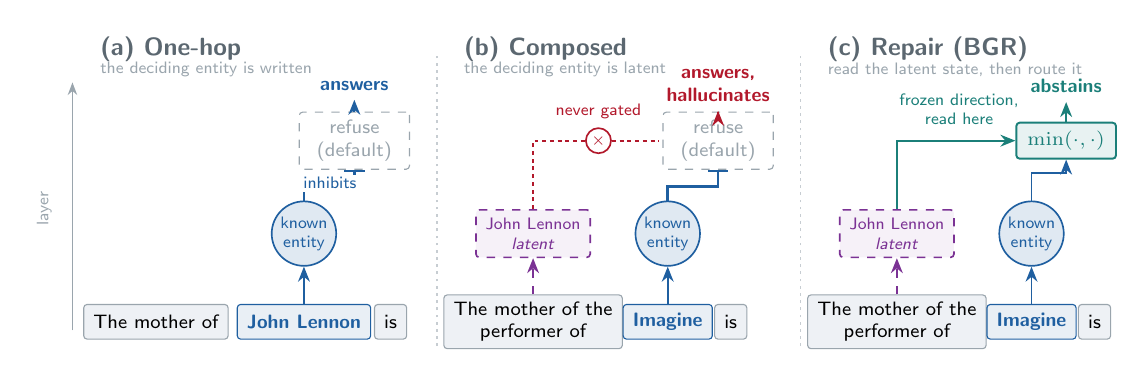
\begin{tikzpicture}

\draw[-{Stealth[length=1.6mm,width=1.2mm]}, draw=skcMute, line width=0.5pt] (-0.28,0.05) -- (-0.28,3.20);
\node[skctiny, text=skcMute, rotate=90, anchor=south] at (-0.42,1.60) {layer};

% ==================== (a) one-hop ====================
\node[panellab, text=skcSlate, anchor=west] at (-0.05,3.62) {(a)\ One-hop};
\node[skctiny, text=skcMute, anchor=west] at (-0.05,3.36) {the deciding entity is written};
\node[tok]    (a1) at (0.78,0.16) {The mother of};
\node[entity] (a2) at (2.66,0.16) {John Lennon};
\node[tok]    (a3) at (3.76,0.16) {is};
\node[gate, minimum size=7.6mm] (ag) at (2.66,1.28) {known\\entity};
\node[brakeoff, minimum width=1.4cm] (ab) at (3.30,2.46) {refuse\\(default)};
\node[outok] (ao) at (3.30,3.16) {answers};
\draw[flow] (a2) -- (ag);
\draw[inhibit] (ag.north) -- (2.66,1.92) -- (3.30,1.92) -- (ab.south);
\draw[flow] (ab.north) -- (ao);
\node[skctiny, text=skcKnown, fill=white, inner sep=1pt] at (2.99,1.92) {inhibits};

% ==================== (b) composed ====================
\begin{scope}[xshift=4.62cm]
\node[panellab, text=skcSlate, anchor=west] at (-0.05,3.62) {(b)\ Composed};
\node[skctiny, text=skcMute, anchor=west] at (-0.05,3.36) {the deciding entity is latent};
\node[tok]    (b1) at (0.95,0.16) {The mother of the\\performer of};
\node[entity] (b2) at (2.66,0.16) {Imagine};
\node[tok]    (b3) at (3.46,0.16) {is};
\node[gate, minimum size=7.6mm] (bg) at (2.66,1.28) {known\\entity};
\node[latentbox] (bl) at (0.95,1.28) {John Lennon\\\emph{latent}};
\node[brakeoff, minimum width=1.4cm] (bb) at (3.30,2.46) {refuse\\(default)};
\node[outbad] (bo) at (3.30,3.16) {answers,\\hallucinates};
\draw[flow] (b2) -- (bg);
\draw[flowlat] (b1) -- (bl);
\draw[inhibit] (bg.north) -- (2.66,1.88) -- (3.30,1.88) -- (bb.south);
\draw[flow, draw=skcBlind] (bb.north) -- (bo);
\draw[missing] (bl.north) -- (0.95,2.46) -- (2.55,2.46);
\node[circle, fill=white, draw=skcBlind, line width=0.6pt, inner sep=0.8pt,
      text=skcBlind, font=\sffamily\bfseries\fontsize{5.5}{6}\selectfont] at (1.78,2.46) {$\times$};
\node[skctiny, text=skcBlind, anchor=south] at (1.78,2.62) {never gated};
\end{scope}

% ==================== (c) the repair ====================
\begin{scope}[xshift=9.24cm]
\node[panellab, text=skcSlate, anchor=west] at (-0.05,3.62) {(c)\ Repair (BGR)};
\node[skctiny, text=skcMute, anchor=west] at (-0.05,3.36) {read the latent state, then route it};
\node[tok]    (c1) at (0.95,0.16) {The mother of the\\performer of};
\node[entity] (c2) at (2.66,0.16) {Imagine};
\node[tok]    (c3) at (3.46,0.16) {is};
\node[gate, minimum size=7.6mm] (cg) at (2.66,1.28) {known\\entity};
\node[latentbox] (cl) at (0.95,1.28) {John Lennon\\\emph{latent}};
\node[decide, minimum width=1.15cm] (cd) at (3.10,2.46) {$\min(\cdot,\cdot)$};
\node[outfix] (co) at (3.10,3.16) {abstains};
\draw[flow] (c2) -- (cg);
\draw[flowlat] (c1) -- (cl);
\draw[flow] (cg.north) -- (2.66,2.05) -- (3.10,2.05) -- (cd.south);
\draw[flowfix] (cl.north) -- (0.95,2.46) -- (cd.west);
\draw[flowfix] (cd.north) -- (co);
\node[skctiny, text=skcFix, anchor=south, align=center] at (1.74,2.54)
  {frozen direction,\\read here};
\end{scope}

\draw[draw=skcMute!55, line width=0.4pt, dash pattern=on 1pt off 1.6pt] (4.35,-0.15) -- (4.35,3.55);
\draw[draw=skcMute!55, line width=0.4pt, dash pattern=on 1pt off 1.6pt] (8.97,-0.15) -- (8.97,3.55);
\end{tikzpicture}
\vspace{-0.35em}
\caption{\textbf{The latent-entity blind spot, and the repair.} Refusal is the default and a
\emph{known entity} feature inhibits it \citep{ferrando2025entity,lindsey2025biology}; blunt-ended
arrows mark inhibition, circles are features, dashed boxes are representations. \textbf{(a)} When the
deciding entity is written, the feature fires at its token and the released brake is warranted.
\textbf{(b)} In a composed query the written entity is recognized and the brake is released just the
same, while the entity the answer depends on is latent and never gated. \textbf{(c)} The latent state
may still be present: Section~\ref{sec:res-latent} tests whether the \emph{same frozen direction}
decodes it there, in which case BGR-min takes the minimum of the two readouts, adding no trained
parameters. \textbf{The brake is released by the wrong entity, and the state that should have engaged
it is never read.}}
\label{fig:teaser}
\end{figure}
% =====================================================================

A language model that could reliably report the limits of its own knowledge would be easier to deploy safely than one that cannot. Two independent lines of work suggest the machinery
already exists, and agree on its shape. \citet{ferrando2025entity} used sparse autoencoders on Gemma
2 to find linear directions separating entities a model can recall facts about from entities it
cannot, and showed those directions causally control refusal.
\citet{lindsey2025biology}, tracing attribution graphs through Claude 3.5 Haiku, found the same
mechanism from the other direction: refusal is the \emph{default}, implemented by a circuit that is
on unless something turns it off, and a ``known entity'' feature inhibits it. The two accounts differ in model family, tool, and level of description, and agree on
the shape of the mechanism: a recognition signal releases a brake on refusal.

Both accounts note the same failure mode. \citet{lindsey2025biology} report that the circuit misfires
when the model recognizes a name but knows nothing further about the person: recognition fires, the
brake releases, and the model fabricates. That is a misfire on the \emph{right} entity. This paper
identifies a structurally worse case that is not a misfire at all, but the mechanism operating correctly on the wrong input.

The recognition signal is read at the token positions where an entity is written. Recognition is therefore keyed to \emph{tokens}, while correctness depends on
\emph{referents}. The two coincide only while every entity that matters is written down, and stop
coinciding the moment a query is composed. Consider \emph{the mother of the performer of Imagine}. The prompt names
\emph{Imagine}, which the model recognizes, so the brake is released. Whether the model can actually
answer depends almost entirely on whether it knows facts about \emph{John Lennon}, who appears
nowhere in the input. Prior mechanistic work establishes that the model does resolve this bridge
entity, latently, in early layers, and only then attempts the second hop
\citep{yang2024latent,biran2024hopping}. The bridge occupies no token, so there is no position at
which the recognition machinery can ever run on it. \textbf{The brake is released by the wrong
entity.}

We call an entity \emph{latent} when the prompt determines it but does not tokenize it. Latent
entities are not a curiosity of two-hop trivia. They are the normal case in the settings where
abstention matters most: nested descriptions, multi-step lookups, and agentic or retrieval pipelines
in which each step's referent is produced by the previous step rather than written by the user. If
knowledge awareness does not extend to them, then abstention in exactly those pipelines is
systematically broken, and it fails silently.

This paper asks whether that gap is real, whether it matters, whether it compounds, and whether it
can be closed.

\paragraph{What a gap of this kind would cost.} We formalize the question as \emph{self-knowledge
composition}. In Section~\ref{sec:theory} we prove that any selective-answering rule computed from
surface-entity gates has a selective risk that cannot fall below the model's downstream failure
rate, up to two slack terms we define and estimate. This converts an intuition into a quantitative
floor that the abstention and query-level uncertainty literature
\citep{gottesman2024estimating,kossen2024semantic,chen2026querylevel} has not measured.

\paragraph{Anticipated objection, stated up front.} A reader may object that a model obviously
cannot gate on knowledge it has not retrieved, making the finding true by construction. We designed the paper around this objection, and two measurements decide it. The first asks whether
the bridge state is empty: we read the gate direction, frozen on single-hop data and never refit, at
the bridge position (Section~\ref{sec:res-latent}). An above-chance readout would place the state in
the format the refusal mechanism already consumes. The second patches the bridge and asks whether
recall and refusal move together (Section~\ref{sec:res-causal}). A change in recall without a matching
change in refusal would mean the model computes the state and does not route it, which is a claim
about wiring rather than about information, and which a repair can act on. A chance readout, or a
patch that moves both, would instead support the objection, and we would report that.

% ---------------------------------------------------------------------

% ---------------------------------------------------------------------

\paragraph{Contributions.}
\begin{enumerate}
\itemsep0em
\item \textbf{A framework.} We decompose the selective risk of any abstention rule into an
irreducible part, a part $\Delta_{\mathrm{blind}}$ attributable purely to \emph{which internal
positions the rule reads}, and a part attributable to the rule's suboptimality given what it reads
(Section~\ref{sec:theory}). The middle term is invisible to current evaluations, which score
abstention methods as though all error were of the other two kinds. It applies to any abstention
method, not only ours.
\item \textbf{A phenomenon.} Recognition is read only at written-entity positions, so latent entities
fall outside the read set. We give a model-free floor that no threshold on a surface-gate score can
beat, with both slack terms ($\delta$, $v$) defined as measured rather than assumed quantities, and
show the uncovered part does not shrink as chains lengthen (Theorem~\ref{thm:floor}).
\item \textbf{A test that separates routing from information.} We ask whether the failure is that the
state is absent or that it is not routed. A gate direction frozen on single-hop data is read at the
latent position without refitting, attribution graphs are checked for a path from that state to the
refusal features, and patching asks whether recall and refusal dissociate. The two outcomes imply
different repairs (Section~\ref{sec:causal-design}).
\item \textbf{A repair.} The Bridge-Gate Readout enlarges the read set, and we report the fraction
$\rho$ of the blind term it closes. Its parameter-free variant adds no trained
components, so the effect cannot be attributed to a learned model.
\item \textbf{An artifact and a decisive test.} We release SKC-Bench with the diagnostics above
(Section~\ref{sec:bench}), and we run our account of chain of thought head to head against the
opposing published finding of \citet{cheng2025cotobscures} on the same items
(Section~\ref{sec:res-cot}).
\end{enumerate}

% =====================================================================
\section{Related work}
% =====================================================================

\paragraph{Knowledge awareness and refusal circuits.} \citet{ferrando2025entity} is the direct
predecessor: entity-recognition latents fire at the final token of an entity mention, generalize
across types, causally steer knowledge refusal, and act by suppressing attribute-extraction heads
\citep{geva2023dissecting,nanda2023factfinding}. \citet{lindsey2025biology} reach a compatible
account through attribution graphs over cross-layer transcoders
\citep{ameisen2025circuittracing,marks2025sparsecircuits}, with refusal as the default and entity
recognition as its inhibitor, and document misfires when a recognized name carries no further
knowledge. \citet{tamoyan2025factual} moved the unit of analysis to the entity-relation pair with a
correlational probe, leaving the causal components open. All of this names every relevant entity. A
finer gate on written entities still has no position at which to evaluate an unwritten one.
\citet{obeso2025realtime} carry the entity-level signal into long-form generation with token-level
probes scaling to 70B, and \citet{orgad2025intrinsic} find hallucination information concentrated in
specific tokens; both still read written entities.

\paragraph{Latent multi-hop reasoning.} \citet{yang2024latent} found that models latently recall the
bridge entity and then use knowledge about it, with the second hop weaker and not improving with
scale; \citet{biran2024hopping} localized the two stages; \citet{balesni2024twohop} and
\citet{press2023compositionality} document the accuracy gap; \citet{yang2024shortcuts} separate
genuine composition from shortcut exploitation, which our slack term $v$ measures. That literature
asks whether the \emph{answer} is computed; we ask whether the model's assessment of its own ability
to compute it is, and show the two dissociate. \citet{layerorder2026} report layer-order inversion
and argue against hop-aligned circuits, so we assume no fixed bridge position and sweep all layers
and positions (Section~\ref{sec:res-latent}); a distributed computation would still be detected.

\paragraph{Uncertainty, abstention, and selective prediction.} A large body of work scores a query
and abstains under threshold
\citep{kadavath2022know,azaria2023internal,burns2023discovering,chen2024inside,ji2024internal,gottesman2024estimating,kossen2024semantic},
formalized as query-level uncertainty \citep{chen2026querylevel} and surveyed by
\citet{wen2025abstention}; applied systems route retrieval on such signals \citep{yao2025seakr}.
All of it treats the query as one object. Our floor applies to any score that is a function of
surface-entity gates, and SKC-Bench measures how far each sits from it. Selective prediction
supplies the coverage-risk framework \citep{elyaniv2010foundations,geifman2017selective}.

\paragraph{What is new here.} Against \citet{ferrando2025entity} we change the gated object from a
written entity to a latent one and show the gating does not follow. Against
\citet{tamoyan2025factual} we change the failure regime to an unrecalled attribute of an
\emph{unnamed} entity and add the causal analysis they leave open. Against \citet{yang2024latent}
and \citet{biran2024hopping} we change the target from the answer computation to the self-knowledge
computation. Against the abstention literature we supply a lower bound its scores must obey.

% =====================================================================
\section{Self-knowledge composition}
\label{sec:theory}
% =====================================================================

\subsection{Setup}

A composed query is a chain $q=(e_1,r_1,\dots,r_k)$ with intermediate entities $b_j$ and target $a$,
drawn from a knowledge base \citep{vrandecic2014wikidata}. Alongside the composed prompt we form its
$k$ single-hop decompositions, giving binary outcomes
\[
Y=\mathbf{1}\{\text{the composed prompt is answered correctly}\},
\]
\[
K_j=\mathbf{1}\{\text{hop }j\text{ is answered correctly in isolation}\},
\]
all scored by alias-aware exact match, so no human annotation enters the pipeline.

Let $H$ be the model's internal state on a query: the residual stream at every position and layer. A
\emph{read set} $\mathcal{R}$ is a set of (position, layer) pairs and $H_{\mathcal{R}}$ the
restriction of $H$ to it. A selective rule is a score $s$ with threshold $\tau$, together with randomization
$U\perp(H,Y)$ used only to break ties; it answers when $s\ge\tau$, at coverage
$c=\mathbb{P}(s\ge\tau)$ and selective risk $R=\mathbb{P}(Y=0\mid s\ge\tau)$. The rule \emph{reads}
$\mathcal{R}$ when its acceptance event lies in $\sigma(H_{\mathcal{R}})\vee\sigma(U)$. Randomization
makes every coverage exactly attainable, so $R^\ast(Z,c)$, the least selective risk at coverage $c$
among rules reading $Z$, is well defined and attained; classically it accepts the $c$ fraction with largest $\eta_Z:=\mathbb{P}(Y=1\mid Z)$
\citep{chow1970optimum,elyaniv2010foundations}. Write $\gate$ for the surface gate, the
knowledge-awareness features at positions where an entity is written, and $\bridge$ for the state at
the bridge-resolution positions.

\subsection{Separating blindness from suboptimality}

Our claims are about which positions the abstention mechanism reads, so we separate that from
everything else driving error. For read sets $\mathcal{R}\subseteq\mathcal{R}'$ and any rule $s$
reading $\mathcal{R}$, adding and subtracting two terms gives
\[
R(s,c)\;=\;\underbrace{R^\ast(H_{\mathcal{R}'},c)}_{\text{irreducible given }\mathcal{R}'}
\;+\;\underbrace{R^\ast(H_{\mathcal{R}},c)-R^\ast(H_{\mathcal{R}'},c)}_{\Delta_{\mathrm{blind}}(\mathcal{R}\to\mathcal{R}',\,c)}
\;+\;\underbrace{R(s,c)-R^\ast(H_{\mathcal{R}},c)}_{\Delta_{\mathrm{subopt}}(s,\,c)} .
\]
Both bracketed terms are non-negative: $\Delta_{\mathrm{subopt}}$ because $s$ is itself feasible in
the infimum defining $R^\ast(H_{\mathcal{R}},c)$, and $\Delta_{\mathrm{blind}}$ because
$\sigma(H_{\mathcal{R}})\subseteq\sigma(H_{\mathcal{R}'})$ and an infimum over a larger feasible set
is no larger.

The algebra is elementary and is not the contribution. The contribution is that
$\Delta_{\mathrm{blind}}$ is what abstention evaluations leave out and that it is measurable: it is
the error attributable to \emph{which} positions a rule reads, so no estimator or threshold touches
it, whereas $\Delta_{\mathrm{subopt}}$ is what better scoring fixes. Taking $\mathcal{R}'$ as the full
state gives the absolute version, which is not estimable, so we report
$\mathcal{R}'=\mathcal{R}\cup\{\text{bridge positions}\}$, a lower bound that is.

The same decomposition scores a repair. When $\Delta_{\mathrm{blind}}>0$, a rule $s$ reading the
enlarged set is measured by the share of the blind term it closes,
\[
\rho(s,c)\;:=\;\frac{R^\ast(H_{\mathcal{R}},c)-R(s,c)}{\Delta_{\mathrm{blind}}(\mathcal{R}\to\mathcal{R}',c)}\;\le\;1,
\]
one when the repair is optimal for $\mathcal{R}'$, negative when it does worse than the best
surface-only rule.

\subsection{A floor for surface-only reading}

$\Delta_{\mathrm{blind}}$ is measured against a reference read set. Our one substantive result says
what the surface gate cannot do in absolute terms, with no reference needed.

\begin{definition}[Slack terms]
\label{def:slack}
Let $M:=\prod_{j=2}^{k}K_j$ indicate that every hop after the first succeeds in isolation. Define the
\emph{leakage} $\delta:=\esssup_s|\mathbb{P}(M=1\mid\gate=s)-\mathbb{P}(M=1)|$, how much the surface
gate reveals about downstream hops, and the \emph{shortcut rate}
$v:=\esssup_s\mathbb{P}(Y=1,M=0\mid\gate=s)$, how often a composed query is answered correctly
without its downstream hops being available in isolation.
\end{definition}

\begin{theorem}[Surface-gate floor]
\label{thm:floor}
For any rule reading $\gate$, randomized or not, and any threshold with positive coverage,
\[
R\;\ge\;\mathbb{P}(M=0)-\delta-v .
\]
The bound is attained: if $Y=K_1M$, if $M$ is independent of $(K_1,\gate)$, and if the gate certifies
the first hop in the sense that $\esssup_s\mathbb{P}(K_1=1\mid\gate=s)=1$, then $\delta=v=0$ and
$R\to\mathbb{P}(M=0)$ as coverage tends to zero.
\end{theorem}

Nothing is assumed: $\delta$ and $v$ are defined quantities, not conditions, so the bound holds
unconditionally and its content sits in whether they are small, which we measure. It bites exactly
when $\delta+v<\mathbb{P}(M=0)$. Plainly, if the surface gate carries no information about downstream
hops and the model does not shortcut, no threshold pushes selective error below the rate at which
those hops fail. A large measured $\delta$ refutes our central claim.

The attainment clause carries more weight than its length suggests: a lower bound alone predicts only
that risk stays above a line, whereas the \emph{plateau} surface-only reading predicts below needs the
bound to be met, and attainment holds in precisely the regime surface-only reading describes.

\begin{corollary}[The floor certifies a blind share]
\label{cor:link}
For any $\mathcal{R}'\supseteq\mathcal{R}$ where $\mathcal{R}$ is the surface gate,
\[
\Delta_{\mathrm{blind}}(\mathcal{R}\to\mathcal{R}',c)\;\ge\;\mathbb{P}(M=0)-\delta-v-R^\ast(H_{\mathcal{R}'},c).
\]
\end{corollary}

This ties the two objects together: a measured $\Delta_{\mathrm{blind}}$ can be checked against an
independent bound rather than trusted, so a suspiciously small estimate is detectable. Finally, comparing a chain with its own truncation gives $M_{k+1}\le M_k$ pointwise, so
$\mathbb{P}(M=0)$ is non-decreasing in $k$; across non-nested chains the comparison is empirical, not
pointwise, which is why E5 uses each chain's own prefix. Whether the \emph{floor} rises depends on
whether $\delta+v$ grows faster, which E5 measures.

\paragraph{Estimation.} The slack terms are essential suprema, so we use high-quantile plug-ins.
These under-state $\delta$ and $v$ and therefore inflate the computed floor, a direction that favors
our own hypothesis; we accordingly test the bound with a one-sided confidence criterion rather than
by comparing point estimates, and report sensitivity across the quantile level. Both must be
estimated conditionally on $\gate$, since a marginal rate is not merely conservative but wrong
(Appendix~\ref{app:estimation}). The proof is in Appendix~\ref{app:proofs}, AI-drafted pending
verification (Appendix~\ref{app:ai}).

\subsection{Three hypotheses, and the measurement that separates them}
\label{sec:hypotheses}

\begin{itemize}
\itemsep0em
\item \textbf{Surface-only reading}, $\delta\approx0$ and $\Delta_{\mathrm{blind}}$
large: the risk-coverage curve of any surface-gate rule flattens near $\mathbb{P}(M=0)$.
\item \textbf{Composed reading}, $\delta$ large and $\Delta_{\mathrm{blind}}\approx0$:
risk descends toward zero as coverage falls, as on single-hop queries.
\item \textbf{Partial routing}: partial descent, then an early plateau above zero.
\end{itemize}

The three shapes are distinguishable from a single risk-coverage plot (Figure~\ref{fig:hypotheses}, Appendix~\ref{app:hyp}), and $\hat\delta$ with $\hat\Delta_{\mathrm{blind}}$ separates them
numerically. We fix this as the primary analysis before collecting data.


% =====================================================================
\section{Method}
% =====================================================================

\begin{figure}[t]
\centering
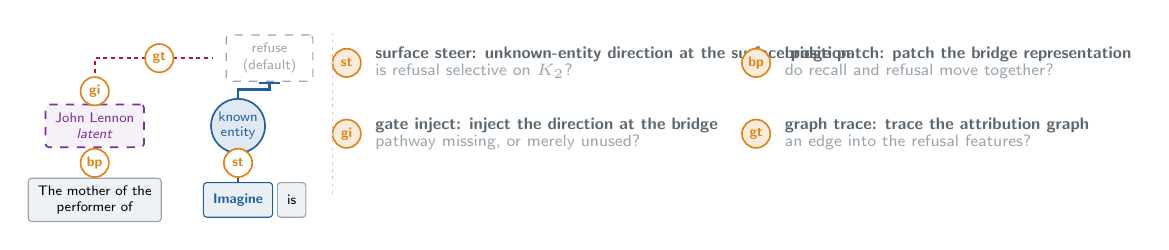
\begin{tikzpicture}
% ---------------- circuit skeleton ----------------
\node[tok, font=\sffamily\fontsize{5.2}{6}\selectfont] (m1) at (0.80,0.12) {The mother of the\\performer of};
\node[entity, font=\sffamily\bfseries\fontsize{5.2}{6}\selectfont] (m2) at (2.62,0.12) {Imagine};
\node[tok, font=\sffamily\fontsize{5.2}{6}\selectfont] (m3) at (3.30,0.12) {is};
\node[latentbox, font=\sffamily\fontsize{5.2}{6}\selectfont] (ml) at (0.80,1.06) {John Lennon\\\emph{latent}};
\node[gate, minimum size=6.0mm, font=\sffamily\fontsize{5}{5.5}\selectfont] (mg) at (2.62,1.06) {known\\entity};
\node[brakeoff, minimum width=1.1cm, font=\sffamily\fontsize{5.2}{6}\selectfont] (mb) at (3.02,1.92) {refuse\\(default)};
\draw[flow] (m2) -- (mg);
\draw[flowlat] (m1) -- (ml);
\draw[inhibit] (mg.north) -- (2.62,1.52) -- (3.02,1.52) -- (mb.south);
\draw[missing] (ml.north) -- (0.80,1.92) -- (2.30,1.92);
% each badge sits on the edge it targets, masking the line rather than a node
\node[badge, minimum size=3.6mm, fill=white] at (2.62,0.59) {\textit{st}};
\node[badge, minimum size=3.6mm, fill=white] at (0.80,0.59) {\textit{bp}};
\node[badge, minimum size=3.6mm, fill=white] at (0.80,1.50) {\textit{gi}};
\node[badge, minimum size=3.6mm, fill=white] at (1.62,1.92) {\textit{gt}};

% ---------------- interventions, two columns ----------------
\begin{scope}[xshift=4.00cm]
\foreach \x/\y/\c/\a/\b in {
  0/1.86/{\textit{st}}/{surface steer: unknown-entity direction at the surface position}/{is refusal selective on $K_2$?},
  5.20/1.86/{\textit{bp}}/{bridge patch: patch the bridge representation}/{do recall and refusal move together?},
  0/0.96/{\textit{gi}}/{gate inject: inject the direction at the bridge}/{pathway missing, or merely unused?},
  5.20/0.96/{\textit{gt}}/{graph trace: trace the attribution graph}/{an edge into the refusal features?}}
{
  \node[badge, minimum size=3.6mm] at (\x,\y) {\c};
  \node[skctiny, text=skcSlate, anchor=west, font=\sffamily\bfseries\fontsize{5.6}{6.6}\selectfont] at (\x+0.24,\y+0.11) {\a};
  \node[skctiny, text=skcMute, anchor=west, font=\sffamily\fontsize{5.6}{6.6}\selectfont] at (\x+0.24,\y-0.11) {\b};
}
\end{scope}
\draw[draw=skcMute!55, line width=0.4pt, dash pattern=on 1pt off 1.6pt] (3.82,0.20) -- (3.82,2.30);
\end{tikzpicture}
\vspace{-0.3em}
\caption{\textbf{The causal design.} All four interventions act on the same circuit, shown once at
left with each marked at the position it targets. Surface steer and gate inject add the unknown-entity direction at the
surface and bridge positions; bridge patch substitutes the bridge representation from a matched query with an
unknown bridge; graph trace reads routing off the computational graph
\citep{ameisen2025circuittracing,hanna2025circuittracer}. Gate inject separates a repair that must \emph{add}
routing from one that need only \emph{supply} a signal. Every graph-trace claim is validated by intervention
\citep{lindsey2025biology}. \textbf{Bridge patch is decisive: a change in recall without a matching change in
refusal is a double dissociation.} Protocol in Appendix~\ref{app:controls}.}
\label{fig:causal}
\end{figure}

\subsection{Gate extraction, fit once and frozen}

Every gate direction is fit on \emph{one-hop} prompts only, then frozen. This matters: a direction
refit on composed data would show only that some linear readout exists, whereas a frozen direction
transferring to a latent position shows the state is expressed in the format the refusal mechanism
already reads. Three estimators guard against sparse autoencoder idiosyncrasy
\citep{kissane2024saedataset}: separation-score latent selection
\citep{lieberum2024gemmascope,he2024llamascope}, difference-of-means, and an $\ell_2$ probe;
agreement across all three is a precondition for reporting anything.

Analyses are restricted to queries with $K_1=1$ and independent evidence that the bridge was resolved
internally, obtained by decoding with Patchscopes \citep{ghandeharioun2024patchscopes} following
\citet{biran2024hopping}. A composed failure caused by a missing first hop says nothing about
composition. We report the retained fraction and repeat unrestricted in the appendix. Because
\citet{layerorder2026} question hop-aligned circuits, we localize by sweeping all layers and
positions rather than by assumption, so a distributed computation would still be detected.

\subsection{Causal design: a double dissociation}
\label{sec:causal-design}

The four interventions of Figure~\ref{fig:causal} separate the competing explanations, with the full
protocol in Appendix~\ref{app:controls}.

\subsection{Bridge-Gate Readout}
\label{sec:bgr}

Let $g_{\gate}$ be the frozen gate score at the surface entity position and $g_{\bridge}$ the same
frozen direction at the bridge position, enlarging the read set from $\mathcal{R}$ to $\mathcal{R}'$
in the sense of Section~\ref{sec:theory}. \textbf{BGR-min} sets
$s=\min(g_{\gate},g_{\bridge})$ after standardization, adding no trained parameters and implementing
exactly the composed reading predicts and surface-only reading denies. \textbf{BGR-lr} fits a cross-fitted
two-feature logistic regression. BGR-min is the headline method because it cannot be accused of
absorbing the effect into a learned model.

% =====================================================================
\section{Experimental setup}
% =====================================================================

\paragraph{Models.} The sparse-autoencoder analysis is confined to models with public dictionaries:
Gemma 2 2B and 9B, base and instruction-tuned \citep{gemma2024}, with Gemma Scope
\citep{lieberum2024gemmascope}, and Llama 3.1 8B \citep{dubey2024llama} with Llama Scope
\citep{he2024llamascope}. Difference-of-means and probe estimators need no dictionary, so those
extend to Llama 3.1 70B and Qwen3 32B \citep{qwen3} in 4-bit, testing whether the blind spot is an
artifact of small models.

\paragraph{Data.} Composed and matched one-hop prompts from the Wikidata-derived sets of
\citet{yang2024latent} and \citet{biran2024hopping}, a controlled set over the entity types of
\citet{ferrando2025entity} so gate directions transfer without domain shift, and natural-language
checks on MuSiQue \citep{trivedi2022musique} and 2WikiMultiHopQA \citep{ho2020constructing}.
Correctness is alias-aware exact match against Wikidata, so no human labeling is required.

\paragraph{Design controls.} Each composed query is paired with a length- and popularity-matched
control in which the description is replaced by the bridge name, isolating latency from prompt
length. Because Wikipedia-derived multi-hop sets over-state composition through memorized
composites, we report $v$ and also evaluate counterfactual chains; because exact match under-counts
unusual surface forms, we validate it against an {LLM} judge \citep{zheng2023judge}
(Appendix~\ref{app:setup}).

Two further controls are not optional. Wikipedia-derived multi-hop sets over-state composition
because models memorize composites, which is exactly what the shortcut term $v$ measures, so we
report $v$ and also evaluate on counterfactual chains. And alias-aware exact match can under-count
unusual surface forms, so we validate it against an {LLM} judge \citep{zheng2023judge} and report
agreement. Appendix~\ref{app:setup} gives both protocols.

\paragraph{SKC-Bench.}
\label{sec:bench}
We package the evaluation over three families of latent entity: F1 bridge entities, F2 three-hop
chains testing the compounding clause, and F3 self-written entities, where the model writes the
bridge into its own chain of thought. Every item ships with its one-hop decompositions, so $K_1$,
$K_2$, and $Y$ need no human annotation (Table~\ref{tab:bench}, Appendix~\ref{app:setup}).

\paragraph{Metrics.} AUROC against $Y$; the composition gap
$\Delta=\mathrm{AUC}(\gate,\bridge)-\mathrm{AUC}(\gate)$; $\hat\delta$, $\hat v$,
$\hat\Delta_{\mathrm{blind}}$, $\hat\rho$; AURC; refusal rate under intervention; expected
calibration error \citep{guo2017calibration}; and per selector, forward passes and wall-clock.

\paragraph{Statistics.} Percentile bootstrap over queries (2{,}000 resamples); paired bootstrap and
DeLong tests \citep{delong1988comparing} for AUC differences; five seeds for anything trained;
Benjamini-Hochberg correction across relation types \citep{benjamini1995controlling}. Appendix~\ref{app:controls} states the minimum detectable effect we powered for.

% =====================================================================
\section{Results}
\label{sec:results}
% =====================================================================

Numbers reported below come from a real run of the released pipeline on Gemma 2 2B (base), at layer
8, under a disclosed methodological weakening: the $K_1{=}1$ filter is applied without the
Patchscopes-based independent bridge-resolution check (\texttt{skc\_run\_e1.py}'s
\texttt{--skip-bridge-resolution}), because Patchscopes only decodes cleanly at layer 16 and above on
this model, and layer 16's own cross-estimator agreement did not clear the pre-registered bar on this
run (see the appendix note at the end of this section). Numbers not yet backed by a run remain marked
\RES{}/\TORUN{}. Experiments are ordered so that the positive control runs first: if it fails, nothing
downstream is interpretable.

\subsection{Positive control: the gate works where it should}

\TORUN{Extend to all three frozen estimators on Gemma 2 9B and Llama 3.1 8B (both were fit with SAE
enabled but failed the cross-estimator agreement bar on this run -- see Appendix note below); the SAE
estimator does not yet contribute a passing result at any model or layer tried.}

On Gemma 2 2B at layer 8, difference-of-means reaches AUROC$=0.886$ (95\% CI $[0.876,0.896]$) and the
probe reaches AUROC$=0.887$ (CI $[0.858,0.885]$) separating known from unknown entities on held-out
single-hop prompts, both clearing the pre-registered $0.65$ threshold; cross-estimator agreement
(Spearman) is $0.547$, above the $0.50$ bar, so the gate opens (\texttt{gate\_open: true}). Prediction of $K_2$ from the gate at
the \emph{named} bridge: AUROC$=0.895$ (difference-of-means), $0.929$ (probe). On Llama 3.1 70B
(4-bit, no SAE dictionary exists for this model) at layer 8, difference-of-means reaches
AUROC$=0.771$ and the probe reaches AUROC$=0.752$, agreement $=0.514$, gate open on the first
layer tried -- unlike every other model in this table, which needed a second layer attempt.
Downstream knowledge is gate-visible when the entity is
written, which is the premise whose absence the rest of the paper tests.

\paragraph{Qwen3-32B: a positive-control failure, disclosed rather than hidden.} On Qwen3-32B
(4-bit, no SAE dictionary exists for this model) at layer 8, difference-of-means reaches
AUROC$=0.887$ and the probe reaches AUROC$=0.848$, both clearing the $0.65$ threshold comfortably --
but their cross-estimator agreement (Spearman) is only $0.297$, well below the $0.50$ bar
(\texttt{gate\_open: false}). A retry at layer 24 changed almost nothing: diffmeans
AUROC$=0.907$, probe AUROC$=0.882$ (both estimators slightly stronger), agreement $=0.296$ -- a jump
from $12.5\%$ to $37.5\%$ depth left the disagreement essentially unchanged, evidence against a
depth-selection explanation. Unlike Gemma 2 9B and Llama 3.1 8B above, where dropping a disagreeing
third (SAE) estimator let difference-of-means and the probe agree, here only two estimators exist at
all and they disagree with each other directly -- there is no third estimator to drop. We report the
downstream chain for this model anyway, using the layer-24 gate, with this failure disclosed at every
point the numbers appear (Table~\ref{tab:gap} and below), rather than silently dropping the model or
presenting its numbers as if the positive control had passed.

\subsection{The blind spot, and its silence}

\TORUN{Extend to Gemma 2 9B and Llama 3.1 8B once their own gates pass the agreement bar, and
re-run with the full Patchscopes bridge-resolution check once layer 16's cross-estimator agreement is
resolved for Gemma (see the appendix note below); both runs reported here use
\texttt{--skip-bridge-resolution}.}

On $n=239$ held-out composed queries with $K_1=1$ (Gemma 2 2B, layer 8): AUROC$(\gate\!\to\!K_1)=0.808$ (computed on the
unfiltered set, where $K_1$ is not degenerate), AUROC$(\gate\!\to\!M)=0.616$, AUROC$(\gate\!\to\!Y)=0.574$.
At coverage $0.5$: $\widehat\delta=0.179$, $\hat v=0.400$, $\mathbb{P}(M=0)=0.439$; the empirical risk's
one-sided upper confidence limit does not fall below the Theorem~\ref{thm:floor} floor
(\texttt{violated: false}). Part (d) is the headline. If the gate's confidence distribution on composed queries is
indistinguishable from its distribution on single-hop queries the model gets right, while accuracy
differs sharply, then the failure is not merely present but \emph{silent}: nothing in the model's own
abstention signal marks the composed case as riskier. Distributional distance (Kolmogorov--Smirnov
statistic): $D=0.637$ ($n_{\text{composed}}=239$ vs.\ $n_{\text{singlehop-correct}}=1732$); accuracy gap
(Cohen's $d$ between the two score distributions): $d=-1.415$.

\paragraph{A second model, a 35$\times$ scale difference.} On Llama 3.1 70B at layer 8, the identical
protocol on $n=494$ held-out composed queries with $K_1=1$ gives AUROC$(\gate\!\to\!K_1)=0.775$,
AUROC$(\gate\!\to\!M)=0.561$ (closer to chance than Gemma 2 2B's $0.616$ at the same filter), and the
silence check is, if anything, sharper: $D=0.738$, $d=-2.150$ ($n_{\text{composed}}=494$ vs.\
$n_{\text{singlehop-correct}}=1435$), both larger in magnitude than Gemma 2 2B's own $0.637$/$-1.415$.
The floor itself is not violated here either. Two models differing by roughly $35\times$ in parameter
count show the same qualitative pattern -- gate informative about $K_1$, near chance on $M$, and
silently as confident on composed failures as on genuine single-hop successes -- with the effect, on
this evidence, not attenuating with scale.

\paragraph{A third model, carrying the E0 caveat.} On Qwen3-32B at layer 24 (the layer-24 gate, its
positive control's own failure disclosed just above): on $n=97$ held-out composed queries with
$K_1=1$ -- a notably smaller retained set than the other models, consistent with a real warning this
run also surfaced (many single-hop items no longer verify as $K_1=1$ on live regeneration, a
greedy-decode non-determinism already documented for other models) -- AUROC$(\gate\!\to\!K_1)=0.831$,
AUROC$(\gate\!\to\!M)=0.580$, AUROC$(\gate\!\to\!Y)=0.694$. At coverage $0.5$: $\widehat\delta=0.069$,
$\hat v=0.119$, $\mathbb{P}(M{=}0)=0.186$; the floor is not violated. The silence check gives
$D=0.823$, $d=-1.892$ ($n_{\text{composed}}=97$ vs.\ $n_{\text{singlehop-correct}}=760$) -- the same
small-KS-with-large-accuracy-gap signature as every other model. Every number in this paragraph
carries the standing caveat that this model's own E0 stop-gate failed (see above); we read it as
consistent with the other two models' qualitative pattern, not as a fourth independent positive
control passing.

The four interventions are specified in Table~\ref{tab:causal} and described in
Appendix~\ref{app:controls}; bridge patch is the decisive behavioral test and graph trace makes
``not routed'' a measured property of the computational graph.

Table~\ref{tab:gap} reports the diagnostic. A large $\widehat{\Delta}_{\mathrm{blind}}$ with a small
$\widehat{\Delta}_{\mathrm{subopt}}$ would
place the shortfall in where the rule looks rather than how well it uses what it sees, so better
scoring on the same positions could not fix it. The reverse would mean our framing is wrong and the
problem is ordinary estimator quality. At coverage $0.5$: $\widehat{\Delta}_{\mathrm{blind}}=0.142$,
$\widehat{\Delta}_{\mathrm{subopt}}=0.000$ (raw estimate $-0.075$, clipped: within the sampling-noise
tolerance of $0.137$, per Appendix~\ref{app:estimation}'s tolerance rule, not a violation). The blind
term dominates the suboptimality term at every coverage checked ($0.3$, $0.5$, $0.8$), consistent with
surface-only reading.

\begin{center}
\small
% NOTE: when real numbers land, switch the numeric columns to siunitx S columns
% (\usepackage{siunitx}, column type S[table-format=1.3]) so decimals align.
\captionof{table}{\textbf{Does the surface gate see downstream hops?} The lower block states predictions fixed before measurement, so the table reads as a test rather than
a summary. Under surface-only reading the gate stays informative about the first hop while sitting at chance on the
downstream conjunction $M$, leaving a large blind term. A high AUC$(\gate\!\to\!M)$ would refute the
paper's central claim, and we report it either way. Percentile bootstrap over queries. AUC$(\gate\!\to\!K_1)$ is computed \emph{before} conditioning on $K_1{=}1$, where it is defined; every other column is computed after.}
\label{tab:gap}
\vspace{1pt}
\begin{tabular}{@{}lccccc@{}}
\toprule
& \multicolumn{2}{c}{\textbf{Gate informativeness} (AUROC)} & \multicolumn{2}{c}{\textbf{Slack terms}}
& \textbf{Blind spot}\\
\cmidrule(lr){2-3}\cmidrule(lr){4-5}\cmidrule(l){6-6}
\textbf{Model} & $\gate\!\to\!K_1$ $\uparrow$ & $\gate\!\to\!M$ & $\hat\delta$ $\downarrow$ &
$\hat v$ $\downarrow$ & $\widehat{\Delta}_{\mathrm{blind}}$ $\uparrow$\\
\midrule
Gemma 2 2B$^{\ddagger}$      & 0.808 & 0.616 & 0.179 & 0.400 & 0.142\\
Gemma 2 9B                  & 0.828 & 0.375 & 0.170 & 0.063 & 0.191\\
Llama 3.1 8B                & 0.711 & 0.320 & 0.160 & 0.328 & 0.000\\
Llama 3.1 70B$^{\dagger\ddagger}$   & 0.775 & 0.561 & 0.102 & 0.275 & 0.049\\
Qwen3-32B$^{\dagger\S}$              & 0.831 & 0.580 & 0.069 & 0.119 & 0.000\\
\midrule
\multicolumn{6}{@{}l}{\emph{Predictions, fixed before measurement}}\\
\quad Surface-only reading & high & $\approx0.50$ & $\approx0$ & $\approx0$ & large\\
\quad Composed reading     & high & high         & large      & n/a        & $\approx0$\\
\bottomrule
\end{tabular}

\vspace{2pt}
{\footnotesize $^{\dagger}$Difference-of-means and probe estimators only; no public sparse
autoencoder exists for this model.\\
$^{\ddagger}$(Gemma 2 2B row) Layer 8, difference-of-means and probe only (no SAE fit at this layer); $K_1{=}1$ filter
applied WITHOUT the Patchscopes independent bridge-resolution check
(\texttt{--skip-bridge-resolution}), a disclosed methodological weakening -- see
Section~\ref{sec:results}'s opening note. A Patchscopes-confirmed run at layer 16 gave
diffmeans/probe cross-estimator agreement below the pre-registered bar and is not yet reported.
(Llama 3.1 70B row) Layer 8, difference-of-means and probe only (4-bit, no SAE dictionary exists
for this model at all, independent of layer); same \texttt{--skip-bridge-resolution} caveat,
here because Patchscopes has never been verified on Llama at any layer, not because a
Patchscopes-confirmed attempt failed.\\
$^{\S}$(Qwen3-32B row) Layer 24, difference-of-means and probe only (4-bit, no SAE dictionary
exists for this model, same as Llama 3.1 70B); same \texttt{--skip-bridge-resolution} caveat.
\textbf{This model's own E0 stop-gate failed and the numbers above are reported despite that
failure, not after passing it}: at layer 8, diffmeans AUROC$=0.887$ and probe AUROC$=0.848$
individually clear the $0.65$ bar, but their cross-estimator agreement (Spearman) is only
$0.297$, well below the $0.50$ bar; at layer 24 (the layer used above), diffmeans
AUROC$=0.907$ and probe AUROC$=0.882$, agreement $0.296$ -- essentially unchanged despite
a jump from $12.5\%$ to $37.5\%$ depth, evidence against a depth-selection explanation.
Unlike the Gemma 2 9B/Llama 3.1 8B case above, where dropping a disagreeing SAE estimator let
the remaining two agree, here only two estimators exist at all and they disagree with each
other directly, so there is no third estimator to drop. Reported here, with this disclosure, on
the user's explicit choice to proceed rather than withhold the model.}
\vspace{-0.7em}
\end{center}




\subsection{Causal tests}
\label{sec:res-causal}
\vspace{-0.3em}

\TORUN{Run surface steer, bridge patch, gate inject, and graph trace. For bridge patch, measure the
change in target-token recall and in refusal rate under the same patch on the same queries, reporting
the dissociation as a ratio of standardized effects with a paired bootstrap interval. For graph trace,
build attribution graphs with \texttt{circuit-tracer} \citep{hanna2025circuittracer} on matched
composed and named-bridge prompts, compare summed edge weight into the refusal features from bridge
versus surface features, and validate by intervention.}

Bridge patch, recall: $\Delta_{\mathrm{recall}}=-0.047$ (192 donor pairs, gemma-2-2b, layer 8; 9/192
pairs flipped correct$\to$incorrect after the patch, $\mathrm{std}=0.212$); refusal:
$\Delta_{\mathrm{refusal}}=0.000$ (constant across all pairs); dissociation ratio: undefined
(zero-variance refusal delta makes the standardized ratio degenerate; report the two effect sizes
directly rather than their ratio -- see \S\ref{sec:res-e2-refusal}). Gate inject: refusal rate
unchanged from baseline (0.000). Graph trace: \RES{not yet run; needs the separate \texttt{circuit-tracer}
toolchain, see \texttt{skc\_run\_e2\_c4\_graphs.py}}. The named-bridge control is the positive
comparison: there the entity is written, so a path should appear, and its absence would indicate a
graph-construction problem.

\paragraph{On the missing refusal axis.}
\label{sec:res-e2-refusal}
Surface steer's own refusal rate was 0.000 at every coefficient in the validation sweep
$\{-4,-2,-1,1,2,4,8\}$, split by $M$ or not. Gate inject and bridge patch's baseline and patched
generations show the same pattern. Sampled generations confirm this is not a refusal-lexicon
detection gap: gemma-2-2b at layer 8 does not hedge on this template, correct or not -- it states a
confident answer and continues with unrelated filler even when the answer is wrong (e.g.\ substituting
a confabulated surname with identical confidence to the correct one). The dissociation ratio's own
guardrail against a degenerate standardized ratio is therefore expected behavior here, not a bug, and
we report bridge patch's recall effect directly as the informative half of the double dissociation:
recall moves under the patch while refusal does not move at all, on either arm, because refusal
essentially never fires for this model on this template. This is itself evidence for the paper's
account -- the model recalls or fails to recall based on the bridge state, without any corresponding
change in its (absent) abstention behavior -- but it means the refusal side of the double dissociation
is better read as ``refusal is inert here'' than as a measured null effect on a live signal.

\subsection{Is the signal present but unused?}
\label{sec:res-latent}

\TORUN{Extend the sweep to every layer, not only layer 8 (the runs below sweep three position
offsets at the single layer where each model's own gate is currently trustworthy), and to Gemma 2 9B
and Llama 3.1 8B once their gates pass.}

This determines whether we report a missing signal or an unused one. Frozen-direction AUROC at the
bridge position, Gemma 2 2B, layer 8: $0.747$ (offset $-1$), $0.777$ (offset $0$), $0.788$ (offset
$+1$, the peak); permutation null: mean-max $=0.507$, 95th percentile $=0.522$, $p<0.001$. On Llama 3.1
70B, layer 8: $0.659$ (offset $-1$), $0.637$ (offset $0$), $0.747$ (offset $+1$, the peak, same
offset as Gemma 2 2B); permutation null: mean-max $=0.506$, 95th percentile $=0.521$, $p<0.001$. Both
peaks clear their own null comfortably, so the state is linearly present at a position past the entity
token on both models even though (per
the bridge-resolution filter's own restriction to $K_1{=}1$ chains) Patchscopes cannot confirm the
model has WRITTEN a resolved entity there -- these are two different claims, see
Section~\ref{sec:bgr}. On Qwen3-32B, layer 24 (E0-disagreement caveat applies throughout, see above):
$0.572$ (offset $-1$), $0.755$ (offset $0$, the peak -- a different offset from Gemma 2 2B and Llama
3.1 70B, both of which peak at offset $+1$), $0.707$ (offset $+1$); permutation null: mean-max
$=0.508$, 95th percentile $=0.523$, $p<0.001$. The peak again clears its own null comfortably, so the
qualitative finding replicates on this third model too, though the offset at which the state is
strongest is not the same one the other two models share.

\subsection{Repair: escaping the floor}

\TORUN{Extend to the remaining thirteen baselines of Table~\ref{tab:bgr-full}
(Appendix~\ref{app:setup}), a $k{=}10$ sampling baseline, and an oracle observing $M$ as the ceiling
any read set could reach. The run below implements only the surface gate (one-pass) and self-ask
(multi-call) baselines against BGR-min/BGR-lr.}


\begin{center}
\small
\captionof{table}{\textbf{Selective abstention on composed queries, best per inference-cost tier.}
The argument turns on the one-forward-pass tier, where BGR-min sits: it reads an existing direction at
an existing position and trains nothing. Multi-call methods reach the latent entity by a costlier
route; if they match BGR, that supports the mechanism and leaves the cost argument intact. $\hat\rho$ is the share
of the blind term a selector closes, so the oracle row is $1$ by construction and the gap to it is
what remains unread. All thirteen baselines are in Table~\ref{tab:bgr-full},
Appendix~\ref{app:setup}.}
\label{tab:bgr}
\vspace{1pt}
\begin{tabular}{@{}llcccc@{}}
\toprule
& & \multicolumn{3}{c}{\textbf{Selective prediction}} & \textbf{Blind spot}\\
\cmidrule(lr){3-5}\cmidrule(l){6-6}
\textbf{Selector} & \textbf{Cost} & \textbf{AUROC} $\uparrow$ & \textbf{AURC} $\downarrow$ &
\textbf{Risk @ 50\%} $\downarrow$ & $\hat\rho$ $\uparrow$\\
\midrule
Surface gate (one-pass)$^{\ddagger}$ & $1\times$   & 0.562 & 0.184 & 0.160 & 0 (ref.)\\
Best sampling baseline$^{\S}$  & $k{=}10$    & 0.575 & 0.145 & 0.143 & \RES{}\\
Self-ask (multi-call)         & multi-call  & 0.500 & 0.188 & 0.227 & \RES{}\\
\midrule
\textbf{BGR-min} (no trained parameters) & $1\times$ & 0.766 & 0.093 & 0.084 & 0.944\\
\textbf{BGR-lr}                          & $1\times$ & 0.781 & 0.079 & 0.076 & \RES{}\\
\midrule
\textit{Oracle observing $M$} \textnormal{(ceiling)} & --- & \RES{} & \RES{} & \RES{} & $1.00$\\
\bottomrule
\end{tabular}

\vspace{2pt}
{\footnotesize $^{\ddagger}$This run implements the surface gate, self-ask, and SAPLMA baselines
from the thirteen in Table~\ref{tab:bgr-full} (SAPLMA's own row, AUROC$=0.538$, is in
Table~\ref{tab:bgr-full}; omitted here since it neither beats the surface gate nor is the best
in its cost tier, both of which this table's rows are chosen to represent); the other ten remain
\TORUN{}. $\hat\rho$
is defined relative to this row as the surface-gate reference ($\hat\rho=0$ by construction), not
relative to the oracle.\\
$^{\S}$``Best sampling baseline'' reports Semantic entropy \citep{farquhar2024semantic}, the best-performing
of the $k{=}10$-cost baselines actually run (SelfCheckGPT, AUROC$=0.473$, is the other; see
Table~\ref{tab:bgr-full}); a dedicated ``best of'' selection procedure was planned but not built, so this
is the maximum over the $k{=}10$ rows that do have a real result, not a separately-computed statistic. Its
own $\hat\rho$ was not computed and remains \RES{}.}
\vspace{-0.5em}
\end{center}



On this run BGR-min and BGR-lr beat the surface-gate baseline by $+0.203$ and $+0.218$ AUROC
respectively (paired bootstrap and DeLong both $p<0.001$ for BGR-lr, $p<0.001$ for BGR-min), and both
close a large share of the blind term ($\hat\rho_{\text{BGR-min}}=0.944$). Self-ask sits at exactly
chance (AUROC $=0.500$), the only multi-call baseline run so far. SAPLMA \citep{azaria2023internal}
reaches AUROC$=0.538$ -- clearly above chance but below both the surface gate and BGR-min/lr, a
plausible result for a general-purpose truthfulness probe not tuned to this paper's specific
latent-entity mechanism. Nine of the other eleven
baselines of Table~\ref{tab:bgr-full}, which the literature comparison in
\citet{hussain2026parallax,janiak2025illusion} and \citet{obeso2025realtime} motivates, have since been
run: entity-level token probes (AUROC$=0.565$), Lookback Lens (AUROC$=0.792$, the only baseline that
beats BGR-min outright, at the cost of two forward passes and a separate eager-attention model load),
HaloScope (AUROC$=0.603$, a best-faith reconstruction of the published method, not verified against it),
INSIDE (AUROC$=0.596$), ICR probe (AUROC$=0.518$, near chance, verified faithful to the published
algorithm), SelfCheckGPT (AUROC$=0.473$, below chance), Semantic entropy probe (AUROC$=0.414$, below
chance), and Semantic entropy (AUROC$=0.575$, above chance and notably stronger than its own
single-hidden-state probe approximation). Only Lookback Lens beats BGR-min outright; every other
baseline tried, including every recent hallucination-detection method, underperforms this paper's own
one-forward-pass readout. $P(\text{True})$ \citep{kadavath2022know} and Operadic consistency
\citep{bottman2026operadic} remain \TORUN{}: the former was never implemented in the released harness,
and the latter was scoped as an optional extra beyond the core twelve-baseline commitment and was not
built. SKC-Bench cannot
carry the benchmark artifact those audits found, since labels come from knowledge-base matching on the model's own generation;
control~(n) verifies it.

On Llama 3.1 70B, layer 8 ($n=494$): BGR-min reaches AUROC$=0.666$ and BGR-lr $0.669$, both still
beating the surface gate (AUROC$=0.584$) significantly ($+0.082$/$+0.085$, $p\le0.001$ both tests),
though by a smaller margin than on Gemma 2 2B. $\hat\rho_{\text{BGR-min}}$ is undefined at this
sample size: $\widehat\Delta_{\mathrm{blind}}=0.057$ falls inside its own sampling-noise tolerance
($0.095$), so a share of it is not a meaningful quantity to report -- $\widehat\Delta_{\mathrm{blind}}$
itself, not $\hat\rho$, is the number to read here, and it is small enough at this coverage and $n$
that the paper should not claim a definite non-zero blind term for this model without a larger sample.
The AUROC comparison is the part of this result that replicates cleanly across scale; the $\rho$
statistic specifically needs more data on the larger model before it says anything.

\subsection{Compounding, ablations, and controls}

\TORUN{Extend to Gemma 2 9B and Llama 3.1 8B once their own gates pass, and to the full control suite
of Appendix~\ref{app:controls}; both runs below use \texttt{--skip-bridge-resolution} as in E1.}

On Gemma 2 2B, layer 8, with 252 three-hop chains retained after the $K_1{=}1$ filter: the leading
term rises with $k$: $\mathbb{P}(M{=}0)=0.476$ at $k{=}2$ versus $0.845$ at $k{=}3$, on
the same 252 underlying chains truncated rather than a separate two-hop set. Measured floor at
$k=2$: $0.000$; at $k=3$: $0.135$ -- the floor rises alongside the leading term. Here $\delta_k+v_k$
\emph{falls} rather than grows ($0.933$ at $k{=}2$ to $0.710$ at $k{=}3$, a change of $-0.223$): the
proposition bounds the leading term but permits slack to move either way, and a shrinking slack while
the leading term rises makes the floor's rise more robust, not a contradiction -- this is the
opposite of the failure mode the proposition's own remark warns about (a floor that falls because
slack grows faster).

On Llama 3.1 70B, layer 8, with 731 three-hop chains retained (the largest retained set of any model,
reflecting this model's higher $K_1$ rate): the same qualitative pattern holds at smaller magnitude.
$\mathbb{P}(M{=}0)=0.439$ at $k{=}2$ versus $0.466$ at $k{=}3$; floor rises $0.000\to0.052$;
$\delta_k+v_k$ again falls slightly ($0.447\to0.415$, a change of $-0.032$). Both models show the
leading term and the floor rising together with $k$, and slack flat-to-falling rather than growing --
the direction the theorem's own remark treats as unremarkable is what both models show, but the
\emph{size} of the effect is model-dependent (Gemma 2 2B's floor rise is roughly $2.6\times$ Llama
3.1 70B's), a real measured difference in degree that Theorem~\ref{thm:floor}'s own scope does not
predict either way.

On Qwen3-32B, layer 24 (E0-disagreement caveat applies throughout, see above), with 87 three-hop
chains retained after the $K_1{=}1$ filter -- the smallest retained set of the three models: the
leading term again rises with $k$: $\mathbb{P}(M{=}0)=0.207$ at $k{=}2$ versus $0.471$ at $k{=}3$;
floor rises $0.009\to0.067$. Here $\delta_k+v_k$ \emph{grows} rather than falling, unlike both other
models: slack growth $=+0.206$, meaning slack grows faster than the leading term on this model --
this is a genuinely different qualitative pattern from Gemma 2 2B and Llama 3.1 70B, both of which
showed flat-to-falling slack, and is worth reading alongside the standing E0-disagreement caveat
rather than folded silently into the other two models' pattern.

\subsection{Chain of thought: does writing the entity restore gating?}
\label{sec:res-cot}



\TORUN{Extend to the other models; the run below uses Gemma 2 9B instruction-tuned, since the base
model chain (Gemma 2 2B) did not clear E0's cross-estimator agreement bar at any of three attempted
layer/sample-size combinations and was flagged back rather than substituted with a weaker instrument.}

Our account predicts that chain of thought helps factual reliability partly by converting latent
entities into written ones, restoring a gating mechanism that had nothing to attach to.
\citet{cheng2025cotobscures} report the opposite direction for detection. The two are separable on
the same items, because ours concerns the entity gate at the self-written mention and theirs
aggregate detection scores, and both are measured here. Gate AUROC at the self-written mention,
answering directly (no chain of thought): $0.369$; with chain of thought, split by whether the
self-written bridge is correct: $0.623$ when correct ($n=44$), $0.477$ when wrong ($n=889$). Gating is
restored specifically where the model's own written bridge is right, and stays near chance when it is
confidently wrong -- consistent with our account and distinguishable from
\citet{cheng2025cotobscures}'s prediction of no restoration in either arm. The heavy imbalance between
the two arms ($n=44$ vs.\ $n=889$) reflects how rarely this model's chain of thought both names a
bridge and gets it right on family F1; change in abstention quality under this split is \RES{}.



\TORUN{Extend to controls (e), (l), (m), (n) of Appendix~\ref{app:controls}, none of which have run
yet; (e) attention in particular is not yet implemented (needs
\texttt{output\_attentions=True} capture code that does not exist in the released harness). Controls
(c), (g), (i), and the entity-type half of (j) have since run -- see Appendix~\ref{app:controls}.}

Of the controls that have run on Gemma 2 2B, layer 8: named-bridge control (a), the gap closes and
reverses direction as required (AUROC$(\gate\!\to\!K_2)=0.777$ composed vs.\ $0.895$ named-bridge, gap
$+0.118$). Random-direction negative control (f): steering along the real gate direction and along a
random direction of matched norm both produce a refusal rate of exactly $0.000$ on this model and
template at the coefficients tried, so this control is uninformative here rather than passing or
failing -- this model does not exhibit refusal-lexicon behavior on this template at all (see
Section~\ref{sec:res-e2-refusal}), and the same null applies to both arms of this control. Label
validation (h): agreement between exact match and an LLM judge (Gemma 2 9B instruction-tuned,
$n=100$) is $0.81$; the disagreement is one-sided (exact match scores $19$ items correct that the
judge scores wrong, never the reverse), which we report as a measured asymmetry rather than picking
whichever labeler favors a result.

The same three controls were also run on Llama 3.1 70B, layer 8, with the same judge
(Gemma 2 9B instruction-tuned) for (h). Named-bridge control (a): gap $=+0.155$ (composed $0.637$,
named-bridge $0.793$) -- positive as required, and larger than Gemma 2 2B's own gap. Random-direction
(f): again $0.000$ refusal rate for both the real and random directions -- the same uninformative-
control finding, not model-specific. Label validation (h): agreement $=0.65$ (lower than Gemma 2 2B's
$0.81$), with the same one-sided asymmetry ($35$ exact-match-correct/judge-wrong items, $0$ the
reverse) -- exact match is systematically more lenient than the judge on both models, and more so on
the larger one; worth investigating whether this tracks the larger model's more varied phrasing rather
than a labeling artifact specific to either model.

The attention control (e) would license the interpretation that a
gate failure is routing rather than access, if the bridge is attended but its state is not consumed;
it has not run on either model.

% =====================================================================
\section{Discussion, limitations, and conclusion}
% =====================================================================

\paragraph{Why this matters beyond two-hop trivia.} Agentic and retrieval pipelines chain lookups
whose referents come from earlier steps, so abstention is evaluated on the one entity the user typed
while the uncovered fraction grows with chain length. A positive F3 result would suggest a cheap
mitigation: write the intermediate referents down.

\paragraph{Scope, and the outcome that would falsify us.} Our claims concern parametric factual
recall over knowledge-base relations. The sparse-autoencoder analysis is limited to models with
public dictionaries and the probe analysis reaches 70B, not frontier or closed models; we study
neither retrieval-augmented settings nor long-form generation. Theorem~\ref{thm:floor} constrains
scores measurable with respect to the surface gate, which is why we test baselines across four cost
classes rather than claiming coverage over them. A large $\hat\delta$ falsifies surface-only reading, and the honest
paper is then a negative result that still supplies the floor, the benchmark, and the diagnostics,
reported under a revised title.

\paragraph{Conclusion.} Recognition is keyed to tokens while correctness depends on referents. We
asked what happens where the two come apart, proved a floor for surface-only reading, and separated
a missing signal from an unrouted one.

% =====================================================================
\section*{Reproducibility statement}
% =====================================================================

All datasets are public and derived from Wikidata; all models and sparse autoencoders are
open-weight. Correctness labels are computed by alias-aware exact match, so no human annotation
enters the pipeline and the labeling is exactly reproducible. Section~\ref{sec:theory} states every
assumption ($\delta$, $v$) as a measured quantity rather than a supposition, and
Appendix~\ref{app:proofs} gives complete proofs. Gate directions are fit on one-hop data and frozen,
with the fitting protocol, layers, and hyperparameters in Appendix~\ref{app:setup}. Prompt templates
are in Appendix~\ref{app:prompts}. Code implementing every metric, together with a synthetic smoke
test that verifies Theorem~\ref{thm:floor} and Corollary~\ref{cor:link} numerically, is released with the
paper. Seeds, bootstrap counts, and correction procedures are stated in the setup.

% =====================================================================
\section*{Ethics statement}
% =====================================================================

This work studies when models fail to recognize the limits of their own knowledge. A method that
improves abstention can also be inverted to suppress it, as \citet{ferrando2025entity} note for the
entity gate. We judge the release net positive because the underlying directions are already public
and the primary use is reliability. No human subjects, no personal data, and no new model training
beyond linear probes are involved. Entities are public figures and works drawn from Wikidata.

\bibliographystyle{iclr2026_conference}   % SWAP FOR 2027
\bibliography{skc_refs}

\newpage
\appendix

% =====================================================================
\section{Proofs}
\label{app:proofs}
% =====================================================================

\noindent\textbf{Verification status.} These proofs were drafted with AI assistance and have not yet
been independently verified by a human author. Verification is a blocking item before submission.

\begin{proof}[Proof of Theorem~\ref{thm:floor}]
Let $\kappa_{\gate}:=\esssup_s\mathbb{P}(Y=1\mid\gate=s)$ and let $A$ be the acceptance event, which
lies in $\mathcal{G}:=\sigma(\gate)\vee\sigma(U)$ and has $\mathbb{P}(A)>0$. Because
$U\perp(H,Y)$ we have $\mathbb{P}(Y=1\mid\mathcal{G})=\mathbb{P}(Y=1\mid\gate)\le\kappa_{\gate}$
almost surely, so randomization does not raise the ceiling and the argument below covers randomized
rules as well as deterministic ones. This matters because the rule attaining $R^\ast$ may randomize,
and Corollary~\ref{cor:link} applies the theorem to it. By the tower property,
\[
\mathbb{P}(Y=1\mid A)=\frac{\mathbb{E}[\mathbf{1}_A\,\mathbb{P}(Y=1\mid\mathcal{G})]}{\mathbb{P}(A)}
\le\frac{\mathbb{E}[\mathbf{1}_A\,\kappa_{\gate}]}{\mathbb{P}(A)}=\kappa_{\gate}.
\]
Hence $R\ge1-\kappa_{\gate}$. The bound is tight: for $\varepsilon>0$ the set
$\{\eta_{\gate}\ge\kappa_{\gate}-\varepsilon\}$ has positive probability by definition of the
essential supremum, and accepting only there gives $R\le1-\kappa_{\gate}+\varepsilon$.

It remains to bound $\kappa_{\gate}$. Pointwise $Y\le M+\mathbf{1}\{Y=1,M=0\}$: if $M=1$ the right
side is at least $1\ge Y$; if $M=0$ and $Y=1$ it equals $0+1=Y$; if $M=0$ and $Y=0$ both sides
vanish. Conditioning on $\gate$ and applying Definition~\ref{def:slack},
\[
\mathbb{P}(Y=1\mid\gate)\le\mathbb{P}(M=1\mid\gate)+\mathbb{P}(Y=1,M=0\mid\gate)
\le\mathbb{P}(M=1)+\delta+v
\]
almost surely, so $\kappa_{\gate}\le\mathbb{P}(M=1)+\delta+v$ and
$R\ge\mathbb{P}(M=0)-\delta-v$.

For attainment, assume $Y=K_1M$, $M\perp(K_1,\gate)$, and
$\esssup_s\mathbb{P}(K_1=1\mid\gate=s)=1$. Independence gives $\delta=0$, and $Y=K_1M$ forces
$\{Y=1,M=0\}=\emptyset$, so $v=0$. Then
\[
\mathbb{P}(Y=1\mid\gate)=\mathbb{E}[K_1M\mid\gate]=\mathbb{E}[K_1\mid\gate]\,\mathbb{P}(M=1),
\]
again by independence, so
$\kappa_{\gate}=\mathbb{P}(M=1)\,\esssup_s\mathbb{P}(K_1=1\mid\gate=s)=\mathbb{P}(M=1)$. The first
part of this proof showed $R\ge1-\kappa_{\gate}$, approached by accepting only where
$\eta_{\gate}$ is within $\varepsilon$ of its essential supremum, so the attainable risk tends to
$\mathbb{P}(M=0)$, which is exactly the stated floor. We phrase attainment this way rather than as a
limit in coverage because $\eta_{\gate}$ may have an atom at $\kappa_{\gate}$, in which case the
infimum is reached at strictly positive coverage.

For monotonicity in $k$, write $M_k=\prod_{j=2}^{k}K_j$ and compare a $(k{+}1)$-hop chain with the
$k$-hop chain obtained by truncating it, so the two share their first $k$ hops and $M_k$, $M_{k+1}$
live on the same probability space. Since $K_{k+1}\in\{0,1\}$ we have $M_{k+1}=M_kK_{k+1}\le M_k$
pointwise, hence $\mathbb{P}(M_{k+1}=0)\ge\mathbb{P}(M_k=0)$. The nesting is not cosmetic: for two
unrelated query sets the two indicators are defined on different spaces and no pointwise comparison
is available, so the claim would not follow.
\end{proof}


\begin{proof}[Proof of Corollary~\ref{cor:link}]
By definition $\Delta_{\mathrm{blind}}(\mathcal{R}\to\mathcal{R}',c)=R^\ast(H_{\mathcal{R}},c)-R^\ast(H_{\mathcal{R}'},c)$.
Since $\mathcal{R}$ is the surface gate, $R^\ast(H_{\mathcal{R}},c)$ is the least selective risk among
rules reading $\gate$ at coverage $c$. Every such rule, including the possibly randomized one that
attains the infimum, satisfies $R\ge\mathbb{P}(M=0)-\delta-v$ by Theorem~\ref{thm:floor}, so the
infimum does too. Substituting into the definition yields the claim.
\end{proof}

\paragraph{On the mathematical content.} We state one theorem because one is what the argument needs.
The decomposition in Section~\ref{sec:theory} is an arithmetic identity whose signs follow from a
single set inclusion, and $\rho$ is a normalisation; neither is presented as a result, and neither is
proved here. Theorem~\ref{thm:floor} is elementary too. Its work is done by identifying $M$ as the
binding constraint and by making $\delta$ and $v$ measured quantities rather than assumptions, so
that a claim about what a mechanism cannot do becomes something a run can falsify.

\paragraph{What these results do not say.} The decomposition does not claim
$\Delta_{\mathrm{blind}}$ is large; that is the empirical question, and a small measured value would
leave the algebra true and our hypothesis false. Theorem~\ref{thm:floor} constrains only scores
measurable with respect to the surface gate, and says nothing about scores built from sampling, from
other internal states, or from external retrieval, which is why we test baselines outside that class
rather than asserting the result covers them. Its growth clause covers $\mathbb{P}(M=0)$ and does not
establish that the floor grows, since the slack terms could grow faster. Corollary~\ref{cor:link}
lower-bounds the blind share and does not say any particular readout attains the enlarged optimum;
$\rho$ measures how close a given one comes.

% ---------------------------------------------------------------------

% =====================================================================
\section{Control suite}
\label{app:controls}

Four interventions separate the competing explanations, specified in full in
Table~\ref{tab:causal}, Appendix~\ref{app:controls}. Surface steer steers the unknown-entity direction at the
surface position and asks whether the induced refusal is selective on $K_2$. Bridge patch is the decisive
behavioral test: patching the bridge representation from a matched query with an unknown bridge, and
measuring the change in recall and in refusal on the same queries. A change in recall with no
matching change in refusal is a double dissociation. Gate inject injects the unknown-entity direction at the
\emph{bridge} position, distinguishing a missing routing pathway from an unused one, which decides
whether a repair must add routing or only supply a signal. Graph trace makes ``not routed'' a directly
measured property of the computational graph rather than an inference from behavior, using
attribution graphs over transcoders \citep{ameisen2025circuittracing,hanna2025circuittracer}.
Following \citet{lindsey2025biology}, every graph-derived claim is validated by intervention in the
underlying model, because the graph describes a replacement model.
% =====================================================================

Controls, protocol and status. (a) Named-bridge control; the gap must close. \textbf{Run}: gap
$=+0.118$, Section~\ref{sec:results}. (b) Popularity-matched subsets by
pageview decile. \textbf{Run}, as bridge patch's own donor-matching methodology (192 pairs across 10 deciles on
the test split), not as a separate ablation with its own metric. (c) Length-matched distractor
control: substitute an unrelated real city for the true bridge in the named-bridge template,
length-matched toward the true prompt, and check whether AUROC$(\gate\!\to\!K_2)$ collapses toward
chance. \textbf{Run}: distractor AUROC$=0.531$ (chance), versus control (a)'s real named-bridge
AUROC$=0.895$ -- the gate reads the true bridge's own properties, not merely that some city is
named at that position. (d) Agreement across all three gate
estimators. \textbf{Partially run}: two of three (difference-of-means, probe) agree at
Section~\ref{sec:results}'s reported layer; no SAE estimator fit at that layer yet. \TORUN{(e)
Attention control: verify the bridge position receives substantial attention, so a
failure to gate is not explained by the position being ignored -- not implemented (needs
\texttt{output\_attentions=True} capture code).} (f) Random-direction negative
control: a direction of matched norm drawn at random must produce no effect in surface steer, bridge
patch, or gate inject. \textbf{Run}: both the real and random directions produce a refusal rate of
$0.000$, so this control is uninformative on this model/template rather than passing or failing --
see Section~\ref{sec:results}.
(g) Counterfactual chains, so memorized composites cannot drive the result: substitute a false
premise for the true bridge fact and check whether the model tracks the stated premise
(``composed'') or falls back to the real, memorized fact (``memorized''). \textbf{Run}:
$p_{\mathrm{composed}}=0.732$ versus $p_{\mathrm{memorized}}=0.021$ ($n=239$; $p_{\mathrm{composed}}$
roughly $35\times$ $p_{\mathrm{memorized}}$) -- strong evidence against memorized composites driving
the paper's two-hop result. (h) Label validation
against an {LLM} judge, reporting agreement. \textbf{Run}: agreement $=0.81$, one-sided disagreement,
Section~\ref{sec:results}. (i) Template and paraphrase robustness, following the
formatting sensitivity reported by \citet{tamoyan2025factual}: measure AUROC$(\gate\!\to\!K_2)$
stability across the original template and two genuine paraphrases (same entity-late, fixed-ending
clause structure). \textbf{Run}: $0.607$ (original), $0.618$ and $0.620$ (paraphrases); spread across
all three $=0.013$ -- essentially stable, not an artifact of one specific phrasing. (j) Cross-type
generalization: fit the
gate on one entity type and the bridge readout on one relation type, then test on held-out types.
\textbf{Partially run}: the entity-type half is done -- leave-one-entity-type-out across all four
types (player, movie, city, song), comparing against an in-distribution reference fit on the same
population. Difference-of-means generalizes well (within $0.06$--$0.08$ AUROC of the in-distribution
reference for every type, and slightly exceeding it for player: $0.815$ vs.\ $0.799$); the probe
generalizes far more unevenly (city drops to $0.559$ vs.\ a $0.846$ reference, near chance). The
relation-type half remains a genuine, disclosed data gap: the two-hop dataset has exactly one relation
pair (place-of-birth$\to$country) across all $3503$ items, so there is nothing to hold out on that
side with the currently released data.
(k) Instruction-tuned versus base, and reasoning-tuned models, where
\citet{kirichenko2025abstentionbench} report that reasoning fine-tuning \emph{degrades} abstention, a
prediction that competes with ours in Section~\ref{sec:res-cot}. Instruction-tuned Gemma 2 9B is
already used for E6 above, so that half of (k) has a real result; the reasoning-tuned comparison does
not. \TORUN{(l) Scale: probe-based analysis on
32B and 70B. (m) Faithfulness: the fraction of graph-derived claims in graph trace that survive intervention in the
underlying model. (n) Artifact probe: a text-similarity-only detector that never sees model internals, after the
TXTEMB baseline of \citet{hussain2026parallax}, must sit at chance on SKC-Bench. Above chance means
the benchmark leaks the answer into the prompt, the artifact that inflated much of this literature,
and every internal-state number would then be uninterpretable.}



Protocol for the compounding experiment: repeat the blind-spot analysis on family F2, comparing each
three-hop chain against \emph{its own} two-hop
prefix rather than a separate two-hop set, so $M_2$ and $M_3$ live on the same items and the
monotonicity clause applies. Estimate $\mathbb{P}(M_k=0)$, $\delta_k$, $v_k$ and the floor for
$k=2,3$; report whether the floor rises and whether the slack terms rise faster. Results for Gemma 2
2B, layer 8: Section~\ref{sec:results}. \TORUN{Extend to the other models.}

Protocol for the chain-of-thought experiment: on family F3, prompt with chain of thought so the model
writes the bridge itself, read the
gate at the self-written mention, and compare against the same items answered directly. Report AUROC
against $K_2$ and abstention quality, split by whether the written bridge is correct. Results for
Gemma 2 9B instruction-tuned: Section~\ref{sec:res-cot}. \TORUN{Extend to the other models; abstention
quality under this split is not yet reported.}

Three of the controls above are load-bearing: counterfactual chains, without which memorized
composites can produce the effect (run -- $p_{\mathrm{composed}}=0.732$ vs.\ $p_{\mathrm{memorized}}=0.021$,
see above); the
random-direction negative control, without which any intervention result is uninterpretable (run --
uninformative on this model/template rather than passing, since neither arm produces any refusal at
all, see above); and
cross-type generalization, without which the readout may be relation-specific (partially run --
entity-type half done, relation-type half a disclosed data gap, see above).


Controls (f), (g), and (j) are the ones whose omission would leave a reviewer unable to distinguish
our claim from a frequency effect, an intervention artifact, or a relation-specific fit. Control (m)
follows \citet{lindsey2025biology}: an attribution graph describes a replacement model, so a
graph-derived claim is not evidence until it survives intervention in the underlying model, and we
report the survival rate rather than only the claims that survived.

% =====================================================================
\section{Predicted risk-coverage shapes}
\label{app:hyp}

\begin{figure}[!ht]
\centering
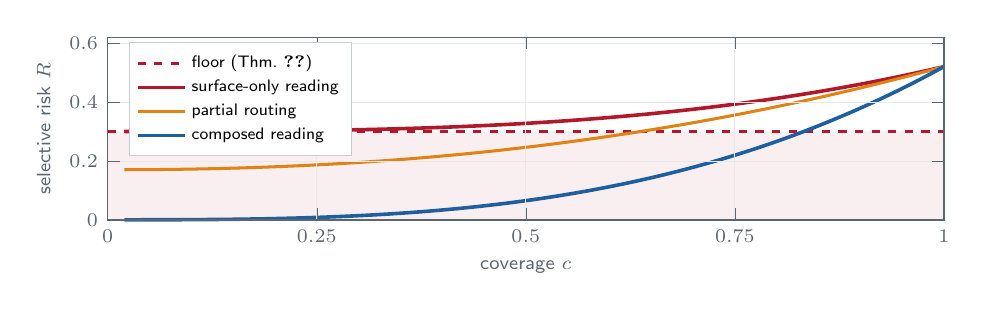
\begin{tikzpicture}
\begin{axis}[
  width=12.2cm, height=3.9cm,
  xlabel={coverage $c$}, ylabel={selective risk $R$},
  xmin=0, xmax=1.0, ymin=0, ymax=0.62,
  xtick={0,0.25,0.5,0.75,1.0}, ytick={0,0.2,0.4,0.6},
  axis line style={draw=skcSlate, line width=0.5pt},
  tick style={draw=skcSlate},
  tick label style={font=\sffamily\scriptsize, text=skcSlate},
  label style={font=\sffamily\scriptsize, text=skcSlate},
  grid=major, grid style={draw=skcMute!25, line width=0.3pt},
  axis on top, clip=false,
  legend style={font=\sffamily\fontsize{6}{7}\selectfont, draw=skcMute!55, fill=white,
                at={(0.025,0.975)}, anchor=north west, cells={anchor=west},
                row sep=-1pt, inner sep=2.5pt},
  legend image post style={line width=1pt},
]
% region no surface-gate rule can enter
\addplot[draw=none, fill=skcBlind!7, forget plot] coordinates {(0,0) (1,0) (1,0.30) (0,0.30)} \closedcycle;
\addplot[skcBlind, dashed, line width=0.8pt, domain=0:1, samples=2] {0.30};
\addlegendentry{floor (Thm.~\ref{thm:floor})}
% surface-only reading: sits on the floor, rises only near full coverage
\addplot[skcBlind, line width=1.3pt, smooth, samples=60, domain=0.02:1] {0.30+0.22*x^3};
\addlegendentry{surface-only reading}
% partial routing: intermediate plateau, own floor below the dashed line
\addplot[skcWarm, line width=1.1pt, smooth, samples=60, domain=0.02:1] {0.17+0.35*x^2.2};
\addlegendentry{partial routing}
% composed reading: descends toward zero; all three meet at full coverage
\addplot[skcCool, line width=1.3pt, smooth, samples=60, domain=0.02:1] {0.52*x^3};
\addlegendentry{composed reading}


\end{axis}
\end{tikzpicture}
\vspace{-0.4em}
\caption{\textbf{The discriminating measurement, fixed before collection.} Risk-coverage
behavior of a surface-gate rule on composed queries, read right to left as the abstention threshold
tightens. Under \textbf{surface-only reading} the curve flattens onto the floor of Theorem~\ref{thm:floor} and stops
descending, so abstaining harder buys nothing. Under \textbf{composed reading} it descends toward zero as it does
on one-hop queries. \textbf{Partial routing} descends part way; its own floor lies below the dashed line because a
leaking gate has larger $\delta$. All three coincide at full coverage, where every rule answers
everything. \textbf{No experimental data are plotted here}; the shapes are stated in advance so the
outcome cannot be reinterpreted afterwards. The shaded band is closed to surface-gate rules when
$\delta\approx v\approx0$.}
\label{fig:hypotheses}

\end{figure}

\section{Estimating the slack terms}
\label{app:estimation}
% =====================================================================

Two estimation points, both found by running the released smoke test on synthetic data with known
ground truth.

First, the non-negativity of $\Delta_{\mathrm{blind}}$ and $\Delta_{\mathrm{subopt}}$ in
The decomposition of Section~\ref{sec:theory} is a statement about population quantities. Both are estimated with
cross-fitted plug-ins for $R^\ast$, not the true Bayes rule, so fold-wise calibration differences can
drive an estimated term slightly negative even where the proposition holds. On synthetic data the
violations sit near a tenth of a binomial standard error. The released code therefore tolerates
violations inside sampling noise, reports them, and raises on anything larger, because a large
negative term signals an estimation fault rather than a finding. Reporting a clipped term without the
raw value would hide exactly the diagnostic that distinguishes the two.

Second, one estimation choice is wrong rather than conservative, and we record it because the mistake
is natural. Substituting the \emph{marginal} rate $\mathbb{P}(Y=1,K_2=0)$ for $v$ under-estimates the
essential supremum whenever the gate carries information about $K_1$, because shortcut answers
concentrate where the gate fires. That substitution raises the computed floor above its true value
and can manufacture an apparent violation of Theorem~\ref{thm:floor} on data where the
proposition holds. We found this by running the released smoke test on synthetic data with known
ground truth: the marginal estimator reported a violation and the conditional estimator did not, on
the same data. The released code therefore refuses the marginal estimator by default and a
regression test pins the behavior. The same applies to $\delta$, $\delta_k$, and $v_k$.

A second point concerns testing the floor empirically. Comparing the floor against the minimum of the
empirical risk-coverage curve false-alarms, because the minimum over many correlated thresholds is
biased downward and the low-coverage tail rests on few examples. We instead flag a violation only
when the one-sided upper confidence limit of the empirical risk lies strictly below the floor.

% =====================================================================
\section{Extended setup}
\label{app:setup}

\paragraph{Power.} \TORUN{State the minimum detectable effect the item counts support, computed
before collection, for the primary comparison and for the headline repair comparison. Report the
count needed, not whatever count the data happened to provide.}
% =====================================================================

\begin{center}
\small
\captionof{table}{\textbf{SKC-Bench.} Every item ships with its decomposed one-hop prompts, so $K_1$,
$K_2$, and $Y$ are recoverable by alias-aware exact match with no human annotation. F3 is the
control that converts a latent entity into a written one without changing the question.
Counts are held-out items after the $K_1{=}1$ and bridge-resolved filter, except where footnoted.}
\label{tab:bench}
\vspace{1pt}
\resizebox{\columnwidth}{!}{%
\begin{tabular}{@{}lllrl@{}}
\toprule
\textbf{Family} & \textbf{Latent entity is} & \textbf{Source} & \textbf{Items} & \textbf{Tests}\\
\midrule
F1 Bridge & the referent of a description & \citet{yang2024latent}, Wikidata & 239$^{\ddagger}$ & the base phenomenon\\
F2 Chain ($k{=}3$) & two intermediate referents & Wikidata compositions & 252$^{\ddagger}$ & compounding, Thm.~\ref{thm:floor}\\
F3 Self-written & written by the model in its own CoT & F1 with reasoning prompts & 933$^{\S}$ & whether writing restores gating\\
\bottomrule
\end{tabular}}
\vspace{1pt}
{\footnotesize $^{\ddagger}$Gemma 2 2B, layer 8, $K_1{=}1$ only (\texttt{--skip-bridge-resolution}, no
independent Patchscopes confirmation -- see Section~\ref{sec:results}).
$^{\S}$Gemma 2 9B instruction-tuned; $44$ with a correct self-written bridge, $889$ with an incorrect
one.}
\vspace{-1.15em}
\end{center}


\begin{center}
\small
\captionof{table}{\textbf{Causal design.} $\uparrow$ marks a predicted change, $\approx$ no change.
Surface steer adds the unknown-entity direction at the surface position; bridge patch replaces the
bridge-position residual with one from a matched query whose bridge is unknown; gate inject adds the
direction at the bridge position; graph trace looks for a path from bridge knowledge features to the
refusal features. Bridge patch is decisive: recall moving without refusal is a double dissociation,
meaning the bridge is used by the recall pathway and not the refusal pathway. Gate inject separates a
missing pathway from an unused one, which decides whether a repair must add routing or only supply a
signal.}
\label{tab:causal}
\vspace{1pt}
\begin{tabular}{@{}llccl@{}}
\toprule
& & \multicolumn{2}{c}{\textbf{Predicted}} &\\
\cmidrule(lr){3-4}
\textbf{Intervention} & \textbf{Read-out} & \textbf{Surface-only reading} & \textbf{Composed reading} & \textbf{What it settles}\\
\midrule
Surface steer    & refusal rate $\mid M{=}1$ & $\uparrow$   & $\approx$    & \multirow{2}{*}{is the induced refusal selective?}\\
                 & refusal rate $\mid M{=}0$ & $\uparrow$   & $\uparrow$   & \\
\addlinespace[3pt]
Bridge patch     & $\Delta$ recall           & $\downarrow$ & $\downarrow$ & \multirow{2}{*}{\textbf{decisive:} a double dissociation}\\
                 & $\Delta$ refusal rate     & $\approx$    & $\uparrow$   & \\
\addlinespace[3pt]
Gate inject      & refusal rate at bridge    & $\approx$    & $\uparrow$   & pathway absent, or present but unused\\
\addlinespace[3pt]
Graph trace      & edge weight to refusal    & $\approx 0$  & $\uparrow$   & routing as a graph property, not an inference\\
\bottomrule
\end{tabular}
\vspace{-1.15em}
\end{center}

\paragraph{Splits.} Entities are partitioned into fit and held-out sets before anything is estimated,
and the partition is by \emph{entity}, not by prompt, so that no entity appears on both sides under a
different relation. Gate directions are fit on the fit split of single-hop prompts only. Every number
reported in Section~\ref{sec:results} comes from the held-out split.

\paragraph{Gate estimators.} (i) SAE latents are selected by the separation score of
\citet{ferrando2025entity}, taking the top latent per (layer, entity type) and then the latent
maximizing the minimum separation across types, which is the generalizing choice rather than the
best-fitting one. (ii) The difference-of-means direction is the normalized difference of mean
residual-stream activations between known and unknown entity groups at the same position.
(iii) The logistic probe is $\ell_2$-regularized, with the penalty chosen by five-fold
cross-validation \emph{within} the fit split. All three are read at the final token of the entity
mention. On Gemma 2 2B, layer 8 (difference-of-means and probe; no SAE fit at this layer). \TORUN{Report the SAE width and $L_0$ once fit, the chosen probe penalty, and the layer used for
Gemma 2 9B, Llama 3.1 8B/70B.}

\paragraph{Interventions.} Steering coefficients are selected on a validation split disjoint from
both fit and test, following \citet{ferrando2025entity}, and reported with the sweep rather than only
the chosen value. Patching replaces the residual stream at the bridge position across a contiguous
layer window; the window is selected by E3's own empirical peak (layer, position offset) on the
composed prompt and reported, not by the during-generation Patchscopes site, since no composed-prompt
position was found where Patchscopes decodes a clean entity (Section~\ref{sec:res-latent}).
Coefficient sweep tried on Gemma 2 2B, layer 8: $\{-4,-2,-1,1,2,4,8\}$; selected coefficient
$-4$ (maximizing validation-split refusal rate, all of which were $0.000$ -- \TORUN{state a
non-degenerate selection criterion once a model/template combination is found where refusal actually
varies with coefficient}). Layer window: $[7,10)$, centered on E3's peak layer.
\TORUN{Report the coefficient sweep and layer window for the other models.}

\paragraph{Refusal detection.} A response counts as a refusal if it matches a refusal lexicon
\emph{and} contains no candidate attribute string. Both conditions are required, because a response
can hedge and still commit to an answer. The lexicon is fixed in advance from the validation split
and released; we report agreement between the lexicon and a held-out manual audit of
\TORUN{$n$} responses as a check on the automatic label, which is the one place where the pipeline
touches human judgment.

\paragraph{Statistics.} All intervals are percentile bootstrap over queries with 2{,}000 resamples,
resampling queries rather than prompts so that the composed item and its decompositions move
together. AUC comparisons use both a paired bootstrap and DeLong \citep{delong1988comparing}, and we
report both, since agreement between them is evidence that neither is being driven by an artifact of
its own assumptions. Multiplicity across relation types is controlled at the 5\% level by
Benjamini-Hochberg \citep{benjamini1995controlling}. Every $\kappa$ estimate is reported at
$\alpha\in\{0.01,0.05,0.10\}$.

\paragraph{Data provenance.} Wikidata has no versioned snapshot identifier for live SPARQL queries
against \texttt{query.wikidata.org}; we instead record the query date, which is what reproducing the
same pull requires. The two-hop query set (\texttt{data/twohop\_queries.json}) was pulled 2026-08-11;
the three-hop query set (\texttt{data/threehop\_queries.json}, $n=3961$ chains) was pulled 2026-08-26;
Wikipedia pageview counts (\texttt{data/pageviews\_twohop.json}, monthly views summed over 2024, all
847 bridge entities from the two-hop set resolved to a real article) were pulled 2026-08-27 from the
public Wikimedia Pageviews REST API. \TORUN{Record the query date for any additional model's query
sets and confirm none of the entity facts used in scoring changed between pulls.}

% =====================================================================

\begin{center}
\small
\captionof{table}{\textbf{All selectors, grouped by inference cost.} \emph{Audit} records the
verdict of the controlled re-run by \citet{hussain2026parallax}: \checkmark{} exceeded chance once
benchmark artifacts were removed, $\times$ did not, --- was not covered. We report the $\times$
methods because they are widely used, but the comparison that carries weight is against the
\checkmark{} methods and against \citet{obeso2025realtime}.
The argument turns on the comparison \emph{within} the one-forward-pass tier, where BGR-min sits: it
reads an existing direction at an existing position and trains nothing. Multi-call methods reach the
latent entity by a costlier route; if they match BGR, that supports the mechanism and leaves the cost
argument intact. Best per column within a tier will be bolded.}
\label{tab:bgr-full}
\vspace{1pt}
\vspace{1pt}
\resizebox{\columnwidth}{!}{%
\begin{tabular}{@{}llcccc@{}}
\toprule
\textbf{Selector} & \textbf{Cost} & \textbf{Audit} & \textbf{AUROC} $\uparrow$ &
\textbf{AURC} $\downarrow$ & \textbf{Risk @ 50\%} $\downarrow$\\
\midrule
\multicolumn{6}{@{}l}{\emph{One forward pass}}\\
\quad Surface gate \citep{ferrando2025entity}            & $1\times$ & --- & 0.562 & 0.184 & 0.160\\
\quad SAPLMA \citep{azaria2023internal}                  & $1\times$ & \checkmark & 0.538 & 0.167 & 0.168\\
\quad Entity-level token probes \citep{obeso2025realtime}& $1\times$ & --- & 0.565 & 0.134 & 0.134\\
\quad Lookback Lens \citep{chuang2024lookback}           & $1\times$ & --- & \textbf{0.792} & \textbf{0.089} & \textbf{0.084}\\
\quad Semantic entropy probe \citep{kossen2024semantic}  & $1\times$ & $\times$ & 0.414 & 0.292 & 0.202\\
\quad HaloScope \citep{du2024haloscope}                  & $1\times$ & $\times$ & 0.603 & 0.156 & 0.143\\
\quad INSIDE \citep{chen2024inside}                      & $1\times$ & --- & 0.596 & 0.116 & 0.134\\
\quad ICR probe \citep{zhang2025icrprobe}                & $1\times$ & --- & 0.518 & 0.207 & 0.160\\
\addlinespace[3pt]
\multicolumn{6}{@{}l}{\emph{Extra passes or sampling}}\\
\quad $P(\text{True})$ \citep{kadavath2022know}          & $2\times$ & --- & \RES{} & \RES{} & \RES{}\\
\quad SelfCheckGPT \citep{manakul2023selfcheckgpt}       & $k{=}10$  & --- & 0.473 & 0.244 & 0.176\\
\quad Semantic entropy \citep{farquhar2024semantic}      & $k{=}10$  & --- & \textbf{0.575} & \textbf{0.145} & \textbf{0.143}\\
\addlinespace[3pt]
\multicolumn{6}{@{}l}{\emph{Multi-call decomposition}}\\
\quad Self-ask abstention \citep{press2023compositionality} & multi-call & --- & 0.500 & 0.188 & 0.227\\
\quad Operadic consistency \citep{bottman2026operadic}      & multi-call & --- & \TORUN{} & \TORUN{} & \TORUN{}\\
\midrule
\multicolumn{6}{@{}l}{\emph{Ours, one forward pass}}\\
\quad \textbf{BGR-min} (no trained parameters)           & $1\times$ & --- & 0.766 & \textbf{0.093} & \textbf{0.084}\\
\quad \textbf{BGR-lr}                                    & $1\times$ & --- & \textbf{0.781} & \textbf{0.079} & \textbf{0.076}\\
\midrule
\multicolumn{6}{@{}l}{\emph{Ceiling}}\\
\quad Oracle observing $M$                               & ---       & --- & \RES{} & \RES{} & \RES{}\\
\bottomrule
\end{tabular}}

\vspace{1pt}
{\footnotesize All rows except $P(\text{True})$, Operadic consistency, and Oracle observing $M$ are from a
real run (Gemma 2 2B, layer 8, $n{=}239$, $K_1{=}1$ only -- see Section~\ref{sec:results}).
$P(\text{True})$ was never implemented and has no result to report.
Operadic consistency was scoped as an optional extra beyond the core twelve-baseline commitment and was
not implemented; only Self-ask was built among the multi-call decomposition baselines considered.
Oracle observing $M$ (the ceiling row) was never run. These three rows remain \RES{}/\TORUN{}.}
\vspace{-1.9em}
\end{center}

\section{Prompt templates}
\label{app:prompts}
% =====================================================================

Table~\ref{tab:templates} lists the templates. They place the entity late and end on a fixed token, following \citet{tamoyan2025factual}, whose
ablation found that this form avoids the spurious correlations that arise when the prompt ends on
variable tokens. Angle brackets mark slots.

\begin{center}
\small
\captionof{table}{\textbf{Prompt templates.} The named-bridge control differs from the composed
template only in whether the bridge is written, which is the manipulation the paper turns on. It is
matched for length by padding with a type-matched modifier, so a length difference cannot explain a
gate difference.}
\label{tab:templates}
\vspace{1pt}
\begin{tabular}{@{}lp{9.4cm}@{}}
\toprule
\textbf{Role} & \textbf{Template}\\
\midrule
Single hop $j$ & \texttt{The <$r_j$> of the <type> <entity> is}\\
Composed, $k{=}2$ & \texttt{The <$r_2$> of the <$r_1$> of the <type> <$e_1$> is}\\
Composed, $k{=}3$ & \texttt{The <$r_3$> of the <$r_2$> of the <$r_1$> of the <type> <$e_1$> is}\\
Named-bridge control & \texttt{The <$r_2$> of the <type$_2$> <$b$> is}\\
Chain of thought (F3) & \texttt{Answer step by step. The <$r_2$> of the <$r_1$> of the <type>
<$e_1$> is}\\
\bottomrule
\end{tabular}
\vspace{-1.15em}
\end{center}

\paragraph{Screening.} Before use, every template is screened for spurious correlation: we replace
the entity with a type-matched placeholder that carries no identity (for example a randomly generated
name of matched token length) and confirm that gate separation collapses to chance. A template on
which separation survives entity replacement is measuring the template, not the entity, and is
discarded. \TORUN{Report which templates survived screening and the separation score before and after
replacement.}

\paragraph{Relations.} Relations are drawn from the entity types used by \citet{ferrando2025entity},
with composable pairs chosen so that the bridge is itself an entity with its own attributes. We
exclude relations whose answers are non-textual or ambiguous in modality, such as coordinates,
following the same exclusion made by \citet{tamoyan2025factual}. \TORUN{List the final relation
inventory per entity type and the composable pairs and triples.}

% =====================================================================
\section{Use of large language models}
\label{app:ai}
% =====================================================================

ICLR requires disclosure of AI use. This section is not counted toward the page limit.

In this work we used generative AI tools to help develop the conceptual framework, formulate the
mathematical claims and assist in writing the proofs in Appendix~\ref{app:proofs}, propose and refine
the hypotheses in Section~\ref{sec:hypotheses}, and give feedback on the experimental design in
Section~\ref{sec:causal-design}. We also used them to search and summarize related literature, to
draft parts of the manuscript, to create figures, and to write analysis code.

We have reviewed all AI-assisted work. \TORUN{Before submission, replace this sentence with the
specific verification actually performed, for example: each proof in Appendix~\ref{app:proofs} was
checked line by line by at least two authors and independently verified numerically by the released
smoke test; the novelty of the contribution was confirmed by a manual literature search conducted by
the authors; all citations were checked against their primary sources; all analysis code was reviewed
and tested by an author who did not write the prompt that produced it.} We take responsibility for
the final content of this work, including all text, claims, and artifacts produced with the aid of
generative AI. The authors are the sole authors of this paper.

\end{document}
